\documentclass{sig-alternate-10pt}
%\input{nsfformat.sty}

%\usepackage{url}
\PassOptionsToPackage{hyphens}{url}\usepackage{hyperref}
\usepackage{wrapfig}
\usepackage{multirow}
\usepackage{times}
\renewcommand{\sfdefault}{phv}
\renewcommand{\rmdefault}{ptm}

%\usepackage[compact]{titlesec}

\usepackage{graphicx}
%\usepackage{subfigure}
\usepackage{subcaption}
\usepackage{stfloats}
\usepackage{listings}
\usepackage{xspace}
\usepackage{comment}
\usepackage{amsmath,amsfonts}

\renewcommand{\baselinestretch}{0.90}

\usepackage{fancyvrb}
\usepackage{fixltx2e}
\fvset{framesep=2mm,fontsize=\scriptsize,framerule=.1mm,numbersep=1mm,commandchars=\\\{\}}
\usepackage[usenames,dvipsnames]{color}

\newenvironment{packed_enum}{
\begin{enumerate}
  \setlength{\itemsep}{1pt}
  \setlength{\parskip}{0pt}
  \setlength{\parsep}{0pt}
}{\end{enumerate}}

\newenvironment{packed_item}{
\begin{itemize}
  \setlength{\itemsep}{1pt}
  \setlength{\parskip}{0pt}
  \setlength{\parsep}{0pt}
}{\end{itemize}}

\newcommand{\eg}{\hbox{\em e.g.}}
\newcommand{\ie}{\hbox{\em i.e.}}
\newcommand{\cf}{\hbox{\em cf. }}
\newcommand{\etal}{\hbox{\em et al.}}
\newcommand{\etc}{\hbox{\em etc.}}

\newcommand{\sysname}{Sensibility Testbed\xspace}

\newif\ifrev
%%%%%%%%%%%%%%%%%%
% COMMENT OUT NEXT LINE TO HIDE TODOs
\revtrue
%%%%%%%%%%%%%%%%%%

\ifrev
  \newcommand{\yanyan}[1]{{\color{blue} [Yanyan: #1]}}
  \newcommand{\cappos}[1]{{\color{red} [Justin: #1]}}
  \newcommand{\albert}[1]{{\color{magenta} [Albert: #1]}}
  \newcommand{\jill}[1]{{\color{Thistle} [Jill: #1]}}
  \newcommand{\lois}[1]{{\color{Peach} [Lois: #1]}}
  \newcommand{\todo}[1]{{\color{red} [TODO: #1]}}
\else
  \newcommand{\yanyan}[1]{}
  \newcommand{\cappos}[1]{}
  \newcommand{\albert}[1]{}
  \newcommand{\jill}[1]{}
  \newcommand{\lois}[1]{}
  \newcommand{\todo}[1]{}
\fi

\usepackage{pifont} 
\newcommand{\tickmark}{\ding{51}}
\newcommand{\xmark}{\ding{55}}

\usepackage{etoolbox}
\apptocmd{\thebibliography}{\setlength{\itemsep}{5pt}}{}{}

% enumerate, etc's margin
%\usepackage{parskip}
%\addtolength{\parskip}{\baselineskip}
\usepackage[neverdecrease]{paralist}
\setdefaultleftmargin{0cm}{}{}{}{}{}

\title{%Reducing Mobile Experimentation Risks with \\Sensibility Testbed:
Balancing Data Acquisition with Privacy Protection \\in Sensibility Testbed}


\author{Yanyan Zhuang$^{\dag, \ddag}$ \and Albert Rafetseder$^{\dag}$ \and Jill Jermyn$^*$ 
\and Justin Cappos$^{\dag}$\\
\and$^{\dag}$New York University \and $^{\ddag}$University of British Columbia \and $^*$Columbia University}

%\email{\small\tt \{doliveir, jnavarro, femilian\}@bowdoin}

% \and \small\tt{crandall@cs.unm.edu}}



%\begin{tabular}{cccc}
%        \multicolumn{1}{c}{Daniela Oliveira} &
%        \multicolumn{1}{c}{Jedidiah Crandall} &
%        \multicolumn{1}{c}{Jesus Navarro}  &
%         \multicolumn{1}{c}{Felix Emiliano}   \\ [.5ex] 
%        \multicolumn{2}{c}{Bowdoin College} &
%        \multicolumn{2}{c}{University of New Mexico } \\ [.5ex] 
%        \multicolumn{2}{c}{{\small\tt \{doliveir, jnavarro, femilian\}@bowdoin.edu}} &
%        \multicolumn{2}{c}{{\small\tt crandall@bowdoin.edu }} &
%\end{tabular}



%}
\date{}

\begin{document}

%\smallskip

\maketitle
\setcounter{page}{1}

%\begin{quote}
%``The world is so full of a number of things'' - that it can be extremely, even hopelessly, confusing. \emph{George Smith, 1945}

%\end{quote}

%\smallskip

\begin{abstract}
%Unfortunately, the expanded use of
%these devices also has lead to increased privacy and security 
%challenges, which makes research on these devices difficult.
%\albert{12 pages, plus unlimited refs. Abstract 250 words max. Due 2015-12-09.}
Due to their omnipresence, mobile devices such as smartphones 
and tablets could be of tremendous value to research. 
However, since research projects can use these devices to collect 
data that reveals personal information, there are substantial
privacy concerns with mobile device use. Therefore, researchers must go through 
a detailed IRB process before recruiting participants.
As such, many research studies either do not use data from real participants or use
data collected from a controlled subset of
participants. %often university students.
%such as investigating end-user traffic patterns, etc. 
%However, the expanded use of mobile 
%devices has resulted in increased privacy and security break-ins 
%on these devices. Therefore, many research institutions require that 
%research on mobile devices must be conducted in a responsible 
%and ethical manner. %challenging for researchers to 
%%conduct research on these devices without compromising
%%the privacy of device owners. 
%This poses challenges to the existing mobile testbeds that 
%play an important role in evaluating network research ideas. 
%The question remains whether research on 
%mobile devices can be carried out using a network testbed, without causing breaches of 
%personal privacy and device security. 

In this paper we present Sensibility Testbed, an experiment  
platform that lowers the policy and technical barriers to performing 
experiments on end users' mobile devices.
%for advancing the use of personal mobile devices in research. 
%security and privacy measures to ensure the 
%The use model of Sensibility Testbed is
%unique in that it (1) manages how device owners make their
%devices accessible to the research community, and (2) offers
%Through the use of a secure sandbox, 
Data can be gathered 
through Sensibility Testbed while reducing the risk of a privacy problem.
%Sensibility Testbed provides privacy protection of mobile device 
%data, and maintains the security of device systems from 
%potentially buggy experiment code. The experiment code in Sensibility 
%Testbed runs in isolated sandboxes to 
%prevent inadvertent or malicious bugs. 
Access to sensor data on a mobile device is mediated according to the policies 
set by the IRB of the researcher's 
institution. These policies are enforced by Sensibility Testbed via technical 
means, not just as stated policies, by a set of non-bypassable 
\textit{blurring layers}. 
Different policies can be created by customizing individual blurring layers 
and loading and stacking them in order on a device. 
These technical innovations simplify the IRB process and allow Sensibility 
Testbed to cater to a wider range of participants. Furthermore, 
Sensibility Testbed's platform design saves researchers' 
effort in recruiting participants and managing a deployment. 
%\cappos{The sentence before this needs to be tightened.  It mentions 
%all sorts of things we don't really cover in the paper.}
Our evaluation shows that \sysname %enables useful experiments to be run
%while 
limits the impact that a buggy or malicious experiment could have on user 
privacy.
%using a combination of blurring and rate-limiting. 
%beyond that of previous campus-only,
%incentivized testbeds, thereby adding to the diversity of the
%installed base in terms of participating devices, OS software
%versions, network operators, participant demographics, countries,
%etc.
%
%experiment measures to researchers that allow them to collect
%data from remote mobile devices without rendering these devices
%at risk. 
%					
%Sensibility Testbed provides privacy mechanisms to protect
%device owners' privacy by mediating data access according to
%researcher's IRB policies. The testbed also uses security
%measures to prevent any inadvertent or malicious bugs in
%experiment code and thus protects the devices. 

%Sensibility Testbed lowers the barriers for researchers to perform
%research experiment on end users' mobile devices, and 
%allows safe research without rendering devices vulnerable.

\end{abstract}


\section{Introduction}

End-user mobile devices, such as smartphones and tablets, have become
indispensable gadgets in people's everyday life. %One study, conducted
%in 2015 by the Pew Research Center
Research has shown that nearly two-thirds of
Americans own a smartphone, and 19\% of them
%in that group observed that 
use the phone as their only means of staying connected~\cite{phone2015}. 
For many people, these devices have become the dominant way they
interact with others, and with the physical world.

Given the sheer number of these devices and the increasing
sophistication of their features,
the value of smart devices as data collection vehicles for government,
university, or corporate studies continues to grow. Since
these devices have embedded GPS,
accelerometers, cameras, and microphones, they can generate valuable
data for such studies as determining noise levels within an urban
neighborhood~\cite{kardous2014evaluation}, detecting approaching 
earthquakes~\cite{faulkner2011next}, or studying traffic
patterns at particular intersections~\cite{zhuang2011time}. Accessing 
devices in a home network can help providers improve the service 
quality~\cite{sundaresan2011broadband}. Testing applications on remote
devices allows developers to better understand how applications 
perform in diverse environments, enabling improvements in 
performance~\cite{ravindranath2012appinsight}. 
%For instance, some platform APIs change their behavior depending 
%on the battery level of the device~\cite{battery}. 
%Without remote access battery life, these APIs can not guarantee basic function efficiency.
%Even being able to
%remotely assess how much life is left in the battery of a device can
%help platform APIs deliver better service to its
%customers~\cite{battery}.
%
As a result, there have been initiatives within the network
community to study mobile devices (e.g.,
Mobilyzer~\cite{nikravesh2015mobilyzer}), and in the systems community
to deploy new services and test research prototypes (e.g.,
Phonelab~\cite{phonelab, nandugudi2013phonelab}). However, personal devices
remain largely underused because of two interrelated challenges:

\begin{itemize}\setlength\itemsep{0em}
\item The risk research studies pose to the privacy of \textbf{device 
owners}, and 

\item The difficulties \textbf{researchers} have
%\cappos{Do you mean obtaining access due to IRB constraints?  What does 
%"securing" mean here?}
obtaining access to devices due to the restrictions set by Institutional Review 
Boards, and using data gathered in a responsible and ethical manner. 
\end{itemize}
					
For device owners, privacy and security threats to mobile devices have
increased dramatically over the years as potential attackers seek
to take advantage of the rich functionality that %and user experience that
sensors\footnote{\scriptsize In this work, we broadly define sensors
as the hardware components that can record phenomena about the
physical world, such as the WiFi/cellular network, GPS location,
movement acceleration, etc.} on mobile devices can provide.
Data acquired through a smartphone's GPS,WiFi
connections, or Bluetooth pairing history can be highly personal,
exposing sensitive information, such as where a person lives or 
shops~\cite{han2012accomplice}. Seemingly benign applications, 
such as popular online games downloaded to mobile devices, can
leak data, such as the model number of the device, or the age, gender, 
or location of its owners~\cite{AngryBirds}. Furthermore, running experiment code poses 
a risk to the operation of the device itself through potential exposure 
to bugs and other vulnerabilities. 
%It can also seriously interfere with battery life, if the device 
%is accessed too often.

For researchers, the challenges are equally formidable. 
Researchers' experiments are under the governance of Institutional 
Review Boards (IRBs)~\cite{irb} that
review all experimental protocols involving human subjects,
and set strict procedures that any researcher working under
the aegis of the institution is required to follow. These include
careful control over the collection and storage of data to ensure the 
privacy of subjects is preserved. It falls on the researcher to enforce 
these policies, and the process must be repeated every time he or 
she starts a new project. 
%The experimenter must also recruit device 
%owners willing to volunteer their devices for testing, 
This process is very time consuming. Moreover, experimental setup 
and results cannot easily be shared with other researchers. 
%As a result, each research group has to repeat the process of 
%infrastructure setup, and policy implementation \cappos{what 
%is this?} for each experimental deployment.

Due to these concerns, experimental testbeds either do not use data 
from real participants (using archived traces like 
in~\cite{kapadia2008anonysense}) or use data collected 
from a controlled subset of participants.
%such as PhoneLab, have been established to provide a platform for 
%running apps on smartphones. 
%PhoneLab recruits participants by giving them free
%smartphones and reduced data plans in exchange for their commitment to
%use the phones as their personal devices. 
%PhoneLab then runs Android apps on the devices and collects data. 
For example, some testbeds deal with both
the recruitment and privacy issues by choosing to select participants
from an internal group, such as faculty working with their students
and colleagues~\cite{hao2013isleep, wang2012no, wang2013sensing}. 
Other testbeds require researchers obtain IRB approval prior to using the
testbed, but provide no technical measures for IRB policy 
enforcement~\cite{phonelab, nandugudi2013phonelab}. 
These mechanisms still fall short, as they do not 
relieve the burden on the researchers to ensure the privacy of the
device owner and to enforce IRB policies. 
%Since the present network testbeds do not yet have a systematic way 
%to provide these protections, there is limited protection for the device 
%owners. 
%Research has shown that most people usually do not understand 
%the basics of privacy, or the implication of granting device
%permissions~\cite{camp2015respecting}. Therefore, if the testbed does 
%not safeguard the security of devices, no matter what 
%advantages participants may receive, their devices are still at risk.
%\cappos{I miss the point of this paragraph in the rest of the narative...}

In this work, we introduce Sensibility Testbed~\cite{sensibility,
zhuang2015privacy}, an Internet-wide mobile testbed that 
%represents an important first step towards 
lowers the technical barriers to research on personal mobile
devices without lowering the ethical standards of the research
institution~\cite{zevenbergen2013ethical}.  
%\cappos{I would instead emphasize 
%that it streamlines IRB since it acts as a middle man for experimenters and 
%participants.  The paragraph here seems to wander to me (e.g., where do we
%discuss ``making prototyping faster'' again?), but eventually comes
%to this point anyways.}
The new testbed streamlines the IRB process for researchers as it acts 
as an intermediate between researchers and device owners. 
%makes experiment prototyping faster, the remote
%control and management of devices easier, and the running of
%experiment code more secure in a number of ways. 
Researchers provide their policy specification to the testbed, and 
the testbed recruits participants and implements the policies on researchers' 
behalf. This model 
makes experiment prototyping faster and more secure in a number of ways. 

First, \sysname provides better protection against invasion of privacy by carefully controlling
access to device sensors. The testbed employs a stringent set of
policies as to which sensors can be accessed, and these
policies are customizable to each researchers' IRB policies. 
%This serves as a template for researchers to parameterize their 
%experiment. 
Second, the testbed infrastructure automatically implements
the IRB policies on end-user devices, through the use of \textit{blurring 
layers} in a secure sandbox. Each blurring layer mediates the access to 
a sensor by limiting the precision of data generated by it, by 
regulating the frequency that the sensor can be accessed, or both. Policy thus
can be easily enforced at the end-user devices by the testbed 
infrastructure. In addition, 
the testbed's secure sandbox provides both security and performance 
isolation, and ensures experiment code cannot harm the devices of 
volunteers. Due to these privacy and security mechanisms, 
the enrollment process for volunteer device owners is as
simple as a one-time download and install of an app, 
%The testbed thus builds and maintains a pool of willing participants for 
%researchers to choose from, 
thus eliminating the time-consuming process of recruitment.


The contributions of this work are as follows:

\begin{itemize}\setlength\itemsep{0em}
%\item We identify the issues that have prevented successful implementation
%of experiments on remote user devices, including potential damage to
%devices from experiment code, the risk of privacy invasion, and the
%administrative challenges faced potential researchers. 

\item We introduce \sysname as a platform for experimentation on 
mobile devices that enables programmable enforcement of 
IRB-approved privacy policies. Our design allows for precise 
programmable control of sensor access through the use of blurring layers 
that substitute approximated data for the more intrusive raw data.

% access to sensor information, including technically enforcing institution-mandated 
%IRB policies. 

\item We integrate a set of baseline privacy policies into the testbed 
design that respond to common attack techniques identified in the 
literature. These policies prevent researchers from maliciously or 
inadvertently accessing private data on personal devices.

%\sysname applies a set of baseline privacy policies that no 
%known attacks would be able to compromise a device. The policies 
%are applied directly on mobile devices. No sensitive information leaves the device.

%\item We describe the unique features of Sensibility Testbed, which include 
%controlled sensor access through the development of blurring layers that are
%highly customizable.

\item To our knowledge, we are the first mobile testbed to prevent 
exfiltration of sensitive information from devices during execution 
without manual intervention by the device owner. 

%\item By greatly reducing the risk to device owners, we encourage 
%greater participation, thus potentially offering researchers a larger and 
%more diverse pool of test subjects.

\end{itemize}

The rest of this paper is organized as follows. In Section~\ref{sec-motivation} we
present background information about several key concepts of \sysname. 
%that are critical to understanding how Sensibility Testbed works and how its use can benefit both researchers and device owners. 
Section~\ref{sec-overview} offers an overview of the basic approval and 
deployment procedure for an experiment. 
%and introduces \sysname's default sensor access policies.
%including a description of its key components and a simplified look at 
The architecture of the Sensibility Testbed 
is reviewed in Section~\ref{sec-design}, and Section~\ref{sec-policy} 
presents the detailed implementation. 
%while Section offers a detailed walkthough of the program in operation. 
Section~\ref{sec-eval} provides experimental results to prove the
viability of Sensibility Testbed in enforcing privacy policies, while
Section~\ref{sec-limitation} examines challenges and current limitations. 
In Section~\ref{sec-related} we review related work,
%in protecting the privacy of data on mobile devices, 
and we share our concluding thoughts in Section~\ref{sec-conclude}.



\section{Motivation and Background}\label{sec-motivation}

In this section, we present some background information on 
factors that shaped the design and deployment of 
Sensibility Testbed. First, we offer the motivations behind its 
development. 
%the desire to balance the benefits of such research 
%with the very real privacy risks that could potentially occur if a 
%device owner allows access to his/her device. 
Next, we look at one solution to the problem of collecting approximate 
data in place of real data. Finally, we talk about 
the traditional role of IRB in research involving human subjects 
and to data accessed remotely. 

\textbf{Motivation: the potential and the risks of accessing sensor data.}
Having access to data from the enormous number of smartphones 
in use today could be tremendously valuable to researchers in a 
number of fields, ranging from health and fitness to the social sciences. 
%One study suggested that collecting sensor-based data is vastly 
%superior to the use of surveys, which can suffer from incomplete 
%content, biases, and a lack of continuity. Because survey-based 
%studies also are "fixed in time," there is no way to monitor behavior 
%over extended periods of time. 
It is also a research method that does not incur high maintenance costs. 
Unfortunately, it is a research method that is ``expensive'' in other ways, 
primarily time. Recruitment of volunteers is time-consuming and often 
frustrating. %There are a number of reasons why this recruitment is so 
%difficult. One is that 
First, %there is no easy method to build a pool of willing participants, 
the recruitment needs to be re-done every time a new experiment is proposed. 
Second, there are complications due to institutional policies on work 
with human subjects (discussed later in this section) that affect who 
can be recruited and under what conditions. An individual recruiting 
on her own is likely to end up with a more homogenous set of subjects, 
drawn either from one locality or interest group. Last but not least, there 
is a very real threat of damage to a participant's device and invasion 
of the participant's privacy. Participants face a significant risk if 
they offer their device to a researcher.

%Due to recent privacy breaches and security break-ins to mobile systems, 
%device security and personal privacy are genuinely at risk when a person 
%uses a smartphone or tablet \cite{breach}. 
%%Apps can post tweets to a 
%%user's Twitter account without asking for permission~\cite{tweet}. 
%A calculator app might send the user's location to an advertisement 
%server~\cite{calc}. Sensor data from the accelerometer 
%or gyroscope can be sufficient to infer the locations of touch-screen 
%taps, and thus infer a user's password~\cite{cai2011touchlogger}.
%Compromised apps can even let criminals break into an individual's 
%bank account~\cite{starbucks}. 
%%As a result, device owners 
%%are aware that running apps on their smartphones can raise privacy 
%%and security risks. 
%A major reason for the prevelant privacy breaches is that on many mobile 
%systems, such as Android, 
%only a sub-set of sensors like GPS and bluetooth are considered risky, 
%and their access is mediated~\cite{android-sec}. Other sensors 
%such as accelerometer, gyroscope, etc., 
%%are considered to be innocuous, 
%require no permission to access. Furthermore, %research shows that 
%device owners are often oblivious to the implications of granting access to
%a particular type of sensor or resource~\cite{felt2012android}. It is 
%therefore challenging to conduct research on end-user devices
%in compliance with ethical standards~\cite{zevenbergen2013ethical}.

%However, having access to data from the enormous number of smartphones 
%in use today could be tremendously valuable to the research 
%community. As these devices belong to ordinary people, conducting
%research on these devices does not incur high maintenance costs. 
%Accelerometers on end-user devices could detect vibrations within 
%the frequency and intensity range of seismic waves, and assist 
%distributed earthquake detection~\cite{faulkner2011next}. GPS, 
%WiFi, and cellular triangulation can be employed in distributed 
%networks of sensors for traffic monitoring and accident 
%prevention~\cite{mohan2008nericell, thiagarajan2009vtrack}. 
%For the research community, accessing this data depends on its 
%ability to provide strong protection to device owners from privacy 
%and security breaches. In this work, we try to address two issues. 

Solutions to the privacy and security problem have been difficult to 
identify, in part because the threat is not broadly recognized by device 
owners. Device owners may not fully 
understand the implications of granting access to a particular type of 
sensor or resource~\cite{felt2012android}. It is therefore challenging to 
conduct research on end-user devices in compliance with ethical standards, 
without an organized approach to enforcing those 
standards~\cite{zevenbergen2013ethical}. Another reason for 
the prevalent privacy breaches on many mobile systems %such as Android and iOS, 
is that only a sub-set of sensors like GPS and Bluetooth are considered risky, 	
and have their access mediated~\cite{android-sec}. Other sensors 
such as accelerometer, gyroscope, etc., require no permission to access, 
thus leaving them open to attack. A first step to expanding the use of sensors on mobile devices is to design solutions that address the security needs of device owners and the practical needs of potential researchers.

\textbf{Restricted data access as privacy protection.}
%Despite these risks of using sensors, 
How specific does data need to be in order to be useful? Studies have indicated that 
sensor data can be accessed without compromising device 
owners' privacy or sacrificing service functioning if that data is generalized. 
Such data that substitutes approximate sensor values does not 
directly violate the privacy of the device owner, and still provides 
valuable information to the researcher conducting the study.
For this reason, researchers have proposed 
substituting mocked~\cite{beresford2011mockdroid} or 
anonymized~\cite{zhou2011taming} data in place of real data. 
For example, in location-based services such as maps, 
restaurant guides, and bus schedules, end users can still use the 
service even if a device only provides a discretized 
location~\cite{amini2011cache, krumm2007inference}. The use of 
generalized data could also encourage more volunteer participation. 
Recent research shows that more than half of the 
surveyed individuals had no problem in supplying imprecise 
sensor data from their personal devices~\cite{fawaz2014location}. 
Most participants could accommodate some reduced application 
functionality, as long as their privacy was protected. Those 
applications included in the survey
ranged from location-based search (e.g., Yelp) and social 
network apps to gaming and weather forecasting apps. 
%the imprecise information is sufficient for a large class of services. \lois{these two sentences have to be clarified. How does one survey an application? And, why would participants be willing to a loss of functionality?}
%The US Federal Communications Commission requires 
%emergency rescue and 
%response teams to be able to estimate a 911 wireless emergency 
%caller's position with an accuracy of 125~m~\cite{gruteser2003anonymous, 
%reed1998overview}. \yanyan{too many examples?}

Based on these facts, restricting 
the amount of data accessible, such as reducing the precision or 
access frequency, offers an effective privacy protection mechanism to 
provide to end users. In this work, we coin the term \textit{data blurring}
as one privacy protection mechanism. However, it must be ensured that  
experiments do not collect more data than they need for providing 
their functionaly. 
An automatic way to substitute approximate data in place of explicit raw data 
is required to achieve realiable and easily usable blurring.


\textbf{IRB policies: guiding ethical behavior.}
%On the other hand, research institutions have also designed a 
%protocol based on the \textit{institutional review board (IRB)}, 
%to assess the ethics of a researcher's project, and review its methods. 
As mentioned earlier, every researcher's work is guided by an 
Institutional Review Board\footnote{\scriptsize Also known as an 
independent ethics committee (IEC), ethical review board (ERB), 
or research ethics board (REB).}, an internal group that serves as 
the ethical watch dogs for colleges, universities, government agencies, 
and other research institutions. It is the job of these boards, 
to approve, monitor, and review research involving human 
subjects~\cite{irb}. 
\begin{comment}
While a commitment to ethical treatment of humans who 
submit to experiments has always been part of the professional codes of most 
scientists, IRBs did not become ubiquitous in research facilities until the 
latter part of the 20th century.  Partly provoked by atrocities committed by 
the Nazis in the name of scientific experiments in the Second World War II, 
and partly inspired by directives from the medical community, including 
Declaration of Helsinki established In 1964 by the World Medical Association, 
research institutions formally acknowledged the need to protect human subjects 
in any research setting. Today, 
\end{comment}
IRBs require all researchers working under 
their aegis to submit the protocols of their studies in advance, with an aim to 
protect not only the physical and mental well-being of subjects, 
but also to protect any information about these individuals generated 
over the course of the study. However, enforcement of these policies becomes significantly harder when dealing with remote subjects. Although many current network 
testbeds require that researchers obtain IRB approval before conducting
an experiment on the testbed, these platforms do not provide a guarantee 
for IRB policy compliance~\cite{nandugudi2013phonelab, nikravesh2015mobilyzer}.
%In the case of PhoneLab, 
%it requires experimenters to obtain IRB approval. However, 
%it leaves it up to the experimenters to comply with their IRB policies in their 
%experiments~\cite{nandugudi2013phonelab, nikravesh2015mobilyzer}. 
%Similarly, Mobilyzer~\cite{nikravesh2015mobilyzer} provides a 
%measurement library that can be included in Android apps. 
%and requires explicit user consent. 
Therefore, there is no guarantee that an 
experiment will be compliant with a researcher's IRB policies. 
%promotes fully informed 
%consent and voluntary participation by prospective subjects. 

%IRB plays a central role in defining the policies
%appropriate for research at individual institutions. Experimenters
%first obtain an IRB approval at their institution. Then with these IRB
%policies, Sensibility Testbed, as an intermediate, codifies the data access 
%regulations and enforces them at the end-user mobile devices. 
%This is achieved through restricting data access  via
%a set of blurring layers. Each layer implements an IRB policy by substituting 
%approximate data in place of explicit, raw sensor data to the experiment code. Different layers 


%Our goal is to facilitate the enforcement of 
%IRB policies on behalf of researchers, and that experiments 
%do not collect more data than needed to provide their functionalities.
%This will also relieve researchers from the tedious work of 
%recruiting participants and enforcing IRB policies.

%In the domain of IRB, Alice and Bob are the participating subject, and 
%a researcher who conducts a research study on the subject, respectively.
%
%
%\textbf{Sensibility Testbed's default policies.}



\section{Overview of Sensibility Testbed}\label{sec-overview}

In this section we discuss the steps required so that experiments 
can run on \sysname. 
%and the researcher's institution's \textit{local IRB}.
%
In the sections below, we present a high-level walkthrough of the steps 
required of the researcher and device owner, and 
introduce how the default policies are designed. 
%We further describe \sysname's design guideline 
%and the resulting testbed components. We also show the testbed operation.
We assume that Alice, a device owner, participates in 
the testbed, while a researcher, Rhonda, wants to runs code on \sysname 
using Alice's device, among other devices.

%\subsection{Walkthrough}\label{sec-walkthrough}

Alice decides to install Sensibility Testbed because she wants to 
altruistically help scientific progress.  She agrees to the privacy
policy for the platform and gives informed consent about the (Section~\ref{subsec:informed-consent})
type of research experiments she wants to participate in.  Alice also
may choose the granularity of data that her phone provides, for 
example to block any possible access to her microphone.  At this point,
her smartphone is ready for researchers to use.  Alice may see experiments 
that are in the approval process, as
well as those that are running on her device, and choose
to opt-out at any time. 

Now suppose that Rhonda, a researcher, wants to study the deployment of
different networking technologies in her city.  She wants to gather
the network type (3G, 4G, LTE, etc.), provider, and signal strength from
users all around the city.  Rhonda goes to the Sensibility Testbed website
and enters information about the sorts of data her experiment requires
into a form (Section~\ref{sec-ch}).  Rhonda decides that she can use randomized IDs in lieu 
of the smarthphone's cell ID, but requires the accurate carrier 
network information such as cellular signal strength and network type. 
%\cappos{please fill in / correct}
She also specifies that her experiment requires GPS data accurate to within
30m for her measurements and needs to update this every 10 seconds.
The Sensibility Testbed website takes her requirements and provides detailed
information for her IRB that Rhonda can use to describe Sensibility
Testbed and how the restrictions that Rhonda agreed to will be technically
enforced.

As is always the case with an IRB, Rhonda's IRB may at this point approve 
or ask her to revise the experiment and its requirements, providing any
changes to the Sensibility Testbed website.  Once approved, Rhonda submits 
the IRB approval to the Sensibility Testbed website.  If 
Rhonda's experiment requests access to sensors in a manner that is 
equal to or at a coarser level than a \emph{baseline} privacy (discussed in more detail
in Section~\ref{sec-policy-design}), her experiment will be immediately approved at this point.
If not, Rhonda's experiment is subject to an additional IRB check at NYU 
to ensure that her experiment will not violate Alice's consent or privacy and
that adequate controls can be put in place to replace the \emph{baseline}
privacy policies (Section~\ref{sec-repy}).

Now approved, Rhonda's experiment can be deployed on end user phones.  She
selects the devices she wishes to use on the Sensibility Testbed 
website, deploys her experiment, and collects the results (Section~\ref{sec-emt}).  
Even if Rhonda's rival Eve steals Rhonda's credentials and deploys a
malicious experiment, the experiment is blocked from accessing sensors except 
in the manner specified in the IRB policy.  Experiment code is blocked from 
reading the WiFi connection information (because this was not requested in
Rhonda's IRB) and is prevented from obtaining Alice's GPS information at a 
finer granularity or frequency than was listed. 
% \cappos{I resisted saying something about battery / malware
%here because these contributions are the focus of other papers.}
Alice is thus happy to let Rhonda perform her experiment, 
knowing that she is contributing to scientific progress without compromising 
her privacy. 
%
%\begin{figure}
%\center{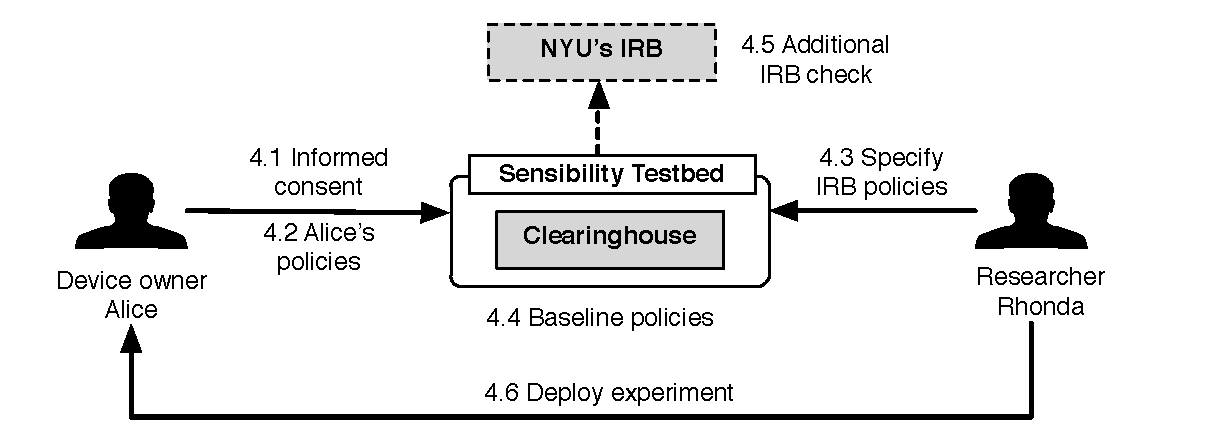
\includegraphics[width=\columnwidth, trim={.9cm .3cm 1.8cm .3cm}, clip]{figs/irb.pdf}}
%%\vspace*{-20pt}
%\caption{\small Overview of \sysname. \label{fig-walkthrough}}
%\end{figure}
%
%The above steps are shown in Figure~\ref{fig-walkthrough}, with each 
%step listed with the corresponding section number. 
This protocol for research with mobile device sensors has been approved by
the IRB at New York University (IRB \# 15-10751).  

\begin{comment}
%For Bob, the steps required to run an experiment include
%on \sysname roughly fall into two categories: 
%IRB approval for his experiment, and code deployment.
%Bob first %designs his experiment, and 
%possibly tests its feasibility on his own device (on which he can 
%use the same \sysname app but does not need IRB approval to access it). 
%Following this, he 
registers his experiment on the \sysname clearinghouse, where he 
specifies the sensors and sensor accuracy that his experiment 
requires through a web form. Suppose that the goal of Bob's experiment is to determine the cellular service
quality in major cities. His experiment therefore needs to obtain location information
of individual devices, their cellular service provider, network
type (3G, 4G, LTE, etc.), and signal strength. 
The clearinghouse's form provides Bob 
%summarizing the request. 
with a list of available sensors and their possible privacy configurations. 
Bob then requests approval for his experiment from his 
institution's IRB, supplying his experiment description using the clearinghouse form, the \sysname's approved 
IRB, and any additional information about the testbed as needed by his institution. 
The process how Bob specifies IRB policies is described in details in 
Section~\ref{sec-ch}. Once Bob's IRB approves the experiment, he 
uploads the confirmation to \sysname's clearinghouse, and is finally 
granted the permission to access devices to deploy his experiment 
and collect data, as will be described in Section~\ref{sec-emt}.

In order for Alice to participate in Sensibility Testbed,
she starts by installing the Sensibility Testbed app from 
the Android app store~\cite{sensibility-app}. After downloading the app, 
Alice is informed about the testbed's privacy and usage policy 
in a consent form and must give consent before participating.
She can opt out of the testbed by uninstalling the app, opt out of
an individual experiment, and set local sensor policies that
will supersede Bob's IRB policies (Section~\ref{sec-repy}). This
protocol for research with mobile device sensors has been approved by
the IRB at New York University (IRB \# 15-10751).  

Bob completes a series of steps to deploy his experiment on \sysname.
He first fills out a form at a \sysname website 
(Section~\ref{sec-ch}), which has a list of checkboxes for device sensors 
and text boxes indicating the precision and frequency that Bob can access 
each sensor. These boxes provide the default policies of \sysname, and 
Bob can only indicate data of coarser granularity. \jill{i thought this process was automated?}
Bob then downloads 
documents to provide to his IRB that 
explains the details about his experiment, \sysname and the technical 
restrictions his experiment will have. Bob then obtains IRB approval at 
his institution, provides his institution's IRB policies to the 
\sysname website, and signs up for his experiment. 

The form that Bob filled out on the \sysname website is used to
enforce a set of technical restrictions for his experiment.  This means
that even if Bob makes an error in his code or his code is malicious, his 
experiment is still restricted in the data it can acquire. 
\yanyan{how can restricting data prevent errors?} Therefore, Bob's IRB 
policies which request access to cellular signal strength and network type, would result 
in his experiment being blocked from reading the cellular roaming status and cell 
IDs. Note that the latter information is accessible with the same 
Android permission, but is blocked by \sysname.  This
protocol for research with mobile device sensors has been approved by
the IRB at New York University (IRB \# 15-10751).  

Note that the policies set limits to the precision of data that Bob can request
for many sensors (e.g., preventing access to the raw MAC address of the device).
If Bob has a legitimate need for this data and can appropriately secure it,
Bob can request such access by also passing his locally approved request 
through \sysname's IRB.  This additional check ensures not only that Bob's 
handling and access to the data is appropriate, but ensures that this does
not violate Alice's privacy and usage policy with the Sensibility Testbed.
%When Bob's IRB wants to access information that is more sensitive than
%what is described in NYU IRB, \yanyan{Justin, help!}  

Once Bob's experiment has been approved and the appropriate privacy
restrictions are identified, Bob can obtain remote devices, and run his experiment on the
devices of participants like Alice (Section~\ref{sec-emt}). On Alice's device, the app displays a 
list of running experiments and their policies. If Alice does not agree with
sharing her MAC address, she can opt out of Bob's experiment. 
%\cappos{how is this updated?  Does Alice see this before or after an 
%experiment may run?  How much "lead time" does Alice get to opt-out
%before the experiment happens?}
%\cappos{Do you want to say something about informed consent here or
%does it fit better later?} 
Alice's informed consent to Sensibility Testbed
ensures that Bob does not need to individually recruit Alice to include
her device in his study.

This work flow is shown in Figure~\ref{fig-walkthrough}. \jill{let's add how Bob gets the 
data from Alice's device in Figure 1} \sysname
acts as an intermediate between the device owner and researcher, 
where the device owners give their informed consent, and researchers
provide their IRB policies. The researchers do not recruit
device owners directly for each experiment, and the testbed infrastructure 
enforces the IRB policies on behalf of the researcher. 

\sysname's default policies are described next.
\end{comment}

%Device owners like Alice participate in Sensibility Testbed by p.

%These policies restrict what and how data can be accessed by the 
%researcher. 
%into data blurring layers that are enforced on
%mobile devices. Such a process can protect device
%owners' personal information. 
%Researchers' code runs in a sandbox that isolates the code from the 
%rest of the device host system. 
%To control the execution of code, Bob uses his own 
%desktop or laptop computer to manage the 
%experiments via the experiment manager. It deploys 
%and runs experiments in sandboxes on remote devices that are 
%acquired through the clearinghouse.

%\textbf{Usage scenario 1: Smartphone owner volunteers as a testbed participant.}
%Alice downloads the Sensibility Testbed app from the Google Play 
%Store~\cite{sensibility-app}, which will install Repy and other software on her phone.
%The app displays a consent form, \yanyan{cite link} containing the testbed's 
%general usage policy. Alice must review and must agree to this 
%policy before installation. If Alice gives her consent, her device will be 
%installed with the Repy sandbox, the native Android code to 
%start or stop the sandbox, and an interface to communicate with the testbed 
%infrastructure (particularly the clearinghouse, described below). 
%By agreeing to our general usage policy, any device 
%owner, regardless of age, country, or background, need only to opt into our testbed as a
%volunteer \textit{once}, at the time of app installation. 
%%As a result, an 
%%researcher like Bob who wants to conduct an experiment 
%%%requests devices through our clearinghouse, which assigns 
%%%them devices from a set of available resources. As a result, 
%%%the researcher
%%does not need to get consent from each subject for each individual
%%experiment. \lois{is the previous sentence needed? I don't think so} 
%The testbed thus greatly simplifies the process for both the 
%device owners and experimenters. 



\section{Sensibility Testbed Architecture}\label{sec-design}

%\cappos{moved here for now.  This may need to be removed altogether.}
The basic operation of \sysname involves three separate 
parties: a \textit{device owner} interested in participating in 
experiments, a \textit{clearinghouse} that discovers the
participating devices, and configures privacy policies on the 
devices,  a \textit{researcher} seeking to run experiments on 
remote devices. 
%As stated in Section~\ref{sec-overview}, the architecture of Sensibility 
%Testbed involves three interacting parties:  
%as shown in Figure~\ref{fig-arch}: 
%researchers, a clearinghouse server, and mobile device owners. 
%discuss the role and functions of each party, and introduce their key 
%techniques. We 
In this section, we use the same example as in 
Section~\ref{sec-overview} to explain the interaction between these 
parties, where researcher Rhonda wants to know the cellular service quality 
using Alice's device.

%\begin{figure}
%\center{\includegraphics[width=\columnwidth]{figs/arch.pdf}}
%%\vspace*{-20pt}
%\caption{\small Sensibility Testbed architecture. \label{fig-arch}}
%\end{figure}

\subsection{Informed Consent}\label{subsec:informed-consent}

After downloading the app, it informs Alice about the testbed's usage and 
privacy policy in a consent form and must give consent before participating.
The consent form~\cite{consent} explicitly notifies the user about the 
types of data that may be collected from their device and how this will
be used for non-advertising research by participating researchers.

%\cappos{Possibly omit, possibly figure...
%
%Sensors that are accessible to experimenters using the Sensibility Testbed 
%report on environmental data around the device, such as temperature, motion, 
%geographic location, etc, but do not snoop on smartphone or network data. For 
%example, no network packet payloads (e.g., your communications with Facebook) 
%or smartphone MAC addresses (e.g., a unique identifier for your phone) will be 
%collected through a WiFi interface. Sensors and types of data collected by a 
%researcher may include: 
%
%\begin{itemize}
%\item Accelerometer, magnetometer, gyroscope, orientation sensors; microphones; etc.
%\item Information about batteries, such as battery technology and level,
%\item Device location using GPS, network, or passive location provider (cached 
%location data on the device);
%\item Network information about Bluetooth, cellular and WiFi connections and 
%the connection quality (data rate, signal strength, etc).   
%\end{itemize}
%
%Researchers use data they collect to examine problems that impact society 
%and perform research experiments. For example, transportation agencies can 
%use sensor data to monitor traffic in an area. Application developers can 
%monitor how programs perform in the field. Wireless network researchers can 
%observe public WiFi and cellular network coverage, and use this information 
%to improve public networks. Environmental scientists might use sensor data 
%to report on the noise level in different areas of a city. 
%}

The policy that a device owner agrees to enables the Sensibility Testbed to
provide access to a researcher to run IRB approved experiments on the device
owner's smartphone.  Each researcher is bound to the IRB agreement of their
experiment and is also bound by the policy of the Sensibility Testbed.  This
means that every researcher does not need to obtain a separate policy with
every experimenter whose device an experiment they will run on.  Instead
each participant only agrees to the policies of the Sensibility Testbed, whose
policies bind the participants together.


The Sensibility Testbed's use policy provides participants the ability
to control how information is gathered from their device. Participants
have the option to opt out of individual experiments, temporary
disable or stop all experiments at any time, and uninstall the 
application at any time.  As we will discuss in the next subsection,
participants also have the ability to control in a more precise manner
how sensors are accessed on the participant's device.

%usage policy requires that the participants in 
%\sysname must be at least 
%18 years old, and do not belong to protected group such as pregnant women.
%Any other device owner, regardless of country or background, can 
%opt into our testbed in this manner, and can opt out just by uninstalling the app. 
%If Alice agrees, the app will be installed on her device, which includes other
%device software that enforces Rhonda's IRB policies specified at the 
%clearinghouse (Section~\ref{sec-bob-policy}), and allows Alice to set her 
%own policies (Section~\ref{sec-alice-policy}).


\subsection{Device Owner's Policies}\label{sec-alice-policy}
A device manager is a part of the device software that 
allows device owners to control the software running on their 
devices. With the device manager, Alice thus can install and remove 
all the other device software, opt in and out of any experiment, 
and set permissions to access the sensors on Alice's device. 

When the \sysname app is started on Alice's device, the device 
manager interface displays a list of running experiments and their policies. If 
Alice does not agree with any policy, she can opt out of the particular 
experiment using the device manager interface. 

Alice can also configure the policies through the device manager to allow
sensors on her device to be acessed at a granularity she is comfortable with.
Alice sets these policies via the user interface of the \sysname app. 
The device manager then parses them just as the clearinghouse
parses Rhonda's IRB policies, and then passes the policies on to the sandbox.
The implementation of Alice's policies is the same as Rhonda's, through
the use of blurring layers.
These policies supersede any policies set by researcher's IRB. For 
example, if Alice disallows access to her location information, then 
Rhonda's experiment cannot get any location from Alice's device even
Rhonda's IRB allows this access. 


\begin{table*}
\scriptsize
\centering

\bgroup
\def\arraystretch{1.15}% % for table padding
\begin{tabular}{|p{3cm}|p{8cm}|p{4cm}|}
\hline
{\bf Privacy concerns\textsuperscript{*}}  & {\bf Sensor data} & {\bf Sensor blurring policies\textsuperscript{\dag}}  
\\ \hline \hline

\multirow{8}{3cm}{N/A} 
& Battery status (charging/discharging), temperature, 
 technology, health (good/overheat), battery level, voltage, plug-in type. & 
 \multirow{8}{4cm}{Full precision, round-up (if numeric), or constant.} \\ \cline{2-2}
 
& Bluetooth scan mode, state (enabled/disabled). &  \\ \cline{2-2}
 
& Cellular network roaming status, SIM card status (ready/absent), 
phone status (idle/busy), signal strength. &   \\ \cline{2-2}

& Location service provider. & \\ \cline{2-2}

& WiFi link speed, association state, nearby routers' frequency, signal strength. & \\ \cline{2-2}
  
& Vibrate mode, screen settings (on/off, brightness, timeout), media/ringer 
volume. &  \\ \hline 

%%%%%%%%%%%%%%%%%%%%%%%%%%%%%%%%%%%%%%

\multirow{2}{*}{Prevent keyloggers.} & Motion sensors: accelerometer, gyroscope, magnetometer, 
orientation, ambient light. & Full precision, round-up, random rotation, constant; restrict 
 access frequency. \\ \hline 

%%%%%%%%%%%%%%%%%%%%%%%%%%%%%%%%%%%%%%

\multirow{12}{*}{Prevent locating a device.} & 
\multirow{3}{*}{Latitude, longitude, altitude.}  & Approximate to the nearest 
zipcode region, or city/state/country center; restrict access frequency.  \\\cline{2-3}
%& & Speed. & Round-up, or constant. & \\\cline{3-4}

& \multirow{2}{*}{Nearby Bluetooth device names.} & Hashed device names; restrict 
 access frequency.  \\ \cline{2-3}

& \multirow{2}{*}{Cellular network cell ID, neighboring cell ID(s).} & Randomized ID; restrict access 
frequency.   \\ \cline{2-3}

& \multirow{2}{*}{Cellular network operator ID and name, country code, area code.} & Hashed ID, names, 
and code; restrict access frequency.  \\ \cline{2-3}

& WiFi connection information (SSID and MAC address of the currently connected router). 
& \multirow{3}{4.1cm}{Hashed SSID, randomized MAC address; restrict 
 access frequency.} \\ \cline{2-2}  
& WiFi scan result (nearby WiFi routers' SSIDs and MAC addresses) & \\ \hline 

%%%%%%%%%%%%%%%%%%%%%%%%%%%%%%%%%%%%%%

\multirow{5}{3cm}{Prevent identifying a device owner.} & \multirow{2}{*}{Bluetooth MAC 
address, local name.}  & Randomized MAC address, hashed device names. \\ \cline{2-3}

& Cellular device ID, incoming number.  & Randomized ID and number. \\ \cline{2-3}

& \multirow{2}{*}{WiFi connection information (device MAC address, IP address).} & 
Randomized MAC address, hashed IP address.  \\ \hline 

%%%%%%%%%%%%%%%%%%%%%%%%%%%%%%%%%%%%%%
%Start/stop activities & & & \xmark \\ \hline 
%Running applications & & & \xmark \\ \hline 
\multirow{2}{*}{Prevent video/ audio recording.} & 
Take pictures, record videosn using a camera. & \multirow{5}{*}{Disabled} \\ \cline{2-2} 

& Voice record using a microphone. & \\ \cline{1-2} 

\multirow{2}{*}{Prevent actions for owner.}& Scan barcode, search, etc., using an Intent.  &  \\ \cline{2-2} 

& Send/receive messages, delete messages, dial/pick up phone calls. & \\  \cline{1-2} 

Protect owner's contacts. & Contact list of the device owner in an address book. & \\ \hline 

\multicolumn{3}{l}{\textsuperscript{*}\scriptsize These goals are the common goals, though uncommon 
goals exist. For example, motion sensors can be used to fingerprint devices~\cite{bojinov2014mobile}, 
or record conversations~\cite{michalevsky2014gyrophone}.} \\ 

\multicolumn{3}{l}{\textsuperscript{\dag}\scriptsize This lists the policies at publication time. They need
to be adjustted as new threats emerge.} \\ 

\end{tabular}
\egroup

\caption{\small Sensibility Testbed's sensor blurring policies for sensor data.}
\label{tab:default}
%\vspace{-10pt}
\end{table*}


\subsection{Researcher Specifies IRB Policies}\label{sec-ch}
Before conducting any experiments, Rhonda first registers an account 
at the clearinghouse. 
The clearinghouse~\cite{ch} is a testbed server that has two 
responsibilities. First, it keeps track of devices and grants 
researchers access to available devices; and second, it
sets up the relevant IRB policies on behalf of the researcher, that 
must be enforced on remote devices.
%It allows experimenters to register accounts and share 
%access to a common pool of devices.

To register his experiment, Rhonda first fills out a form on the clearinghouse 
web page, which has a list of checkboxes for all available sensors 
and text boxes indicating the precision and frequency at which Rhonda 
desires to access 
each sensor. Rhonda checks off only the sensors necessary for his experiment, 
and sets the policies by filling in the text boxes for each sensor.
In this case, Rhonda specifies that 
his experiment can (1) read location information
from devices at the granularity of a city, (2) read accurate
cellular signal strength and network type, as well as
cell IDs, and (3) get location and
cellular network data updates every 10 minutes. 
%Rhonda then downloads documents to provide to his IRB that 
%explains the details about his experiment, \sysname and the technical 
%restrictions his experiment will have. Rhonda then obtains IRB approval at 
%his institution, provides his institution's IRB policies to the 
%\sysname website, and signs up for his experiment. 
After filling out this form, Rhonda downloads the experiment description 
he provided, the detailed information about \sysname's approved IRB, 
and several relevant forms, such as those addressing consent 
(Section~\ref{sec-repy}), terms of participation (for device owners),  
terms of usage (for the researcher), and so on.  
Rhonda then uses these forms as a template to complete the IRB application 
with his institution. These forms serve as a set of reference documents 
to make it easier for researchers like Rhonda to 
file the necessary IRB paperwork with their institutions.

The form that Rhonda filled out on the clearinghouse website is used to
enforce a set of technical restrictions for his experiment. 
The blurring layers are provided by 
\sysname, and are set up in a non-bypassable fashion -- it is not 
Rhonda's task to implement the approved access policies. This means
that even if Rhonda makes an error in his code or his code is malicious, his 
experiment is still restricted in the data it can acquire. 
Therefore, Rhonda's IRB 
policies which request access to cellular signal strength and network type, would result 
in his experiment being blocked from reading the cellular roaming status and area 
code. Note that the latter information is accessible with the same 
Android permission, but is blocked by \sysname. 
After the application is submitted, Rhonda's IRB may disagree with 
his initial experiment requirements. For example, Rhonda's IRB will not permit
his experiment to access cell IDs in cellular networks, but 
approves the other policies. 
%Rhonda wants to access cell 
%IDs in cellular networks, but his IRB disallows such data access. Rhonda then
In this case, Rhonda will revise the experiment registration form, refile the paperwork, 
and obtain IRB approval. Rhonda then submits the revised  
registration form and his IRB approval to the clearinghouse.

 When an account is approved, Rhonda 
% is assigned a pair of public/private \textit{authentication keys} by the 
%clearinghouse, to authenticate himself with the clearinghouse. This
%researcher 
can sign into the clearinghouse and request a 
number of sandboxes for his experiment. The clearinghouse 
looks up available sandboxes on behalf of Rhonda. If Alice's device is discovered, the 
clearinghouse stores her device's meta information (an anonymized 
key), %\textit{identification key}, 
and assigns her device to Rhonda's experiment account. 

The clearinghouse creates a list of sensor access policies for Rhonda's
experiment, according to Rhonda's specified IRB policies. The 
clearinghouse parses Rhonda's registration form, extracts each sensor name, 
data accuracy and access frequency limits as the 
input parameters to the blurring layer code (to blur an exact location 
to a city center, disallow access to cell IDs, and allow cellular network and 
location query once every 10 minutes). Finally, the clearinghouse 
instructs Alice's device to implement these IRB policies. The involvement 
of the clearinghouse in any given experiment ends at this point.
It does not store any data on the researcher's behalf. 

%Besides assigning devices, the clearinghouse also has the role of 
%instructing the sandboxes assigned to this researcher to add the IRB 
%policies specified during registration. The clearinghouse does so 
%by communicating with the resource managers on those devices, which 
%control the code executed in the sandboxes. 

%However, it can direct the release of data to a server designated by the 
%researcher. To do so, the experimenter must register
%his server by providing its certificate and URL to the
%clearinghouse, which will then instruct the devices
%accessible to the experimenter that all the sensor data collected should be
%sent to this server. The sandboxes on these devices will issue
%\texttt{HTTPS POST} using the server's certificate, and send encrypted
%data to the experimenter's server.

%The key role of this component is to facilitate device sharing, 
%which relieves individual experimenters from repeatedly 
%recruiting devices for each experiment.
%
%Note that in Sensibility Testbed, there are two types of keys. A device
%owner has an \textit{identification key} to identify the app installed on a 
%device. This key is mostly used by a lookup service. 

%This pair of keys are mostly used by the clearinghouse and 
%experiment manager.

%\lois{have you introduced the idea of keys yet? If not, I think this needs to be explained.}

\subsubsection{Sensor Blurring Policies}\label{sec-policy-design}

Policies govern at which accuracy and rate a sandboxed experiment can 
access sensors on a device, if any. 
The goal of \sysname is to protect the device owner's privacy, while making
the data from mobile devices useful for a wide range of research. 
%As mentioned earlier, failure to recognize the vulnerability of
%certain sensors was a key reason for privacy breaches. 
Sensibility Testbed uses \textit{default policies} to specify how 
different types of sensors can be accessed to prevent common privacy and
security attacks, %To privide such protection, \sysname 
%classifies sensors as 
%of low, moderate, or high risk. Sensors of high risk are not accessable to 
%researchers by default, and the sensors of low and moderate risk are further 
%protected by the default policies.
%uses a set of policies to prevent a range of attacks, 
as listed in Table~\ref{tab:default}. 
%These policies roughly fall into three categories.
Researchers can further customize the policies through their IRB
to access sensors at a coarser data granularity. The default and 
customized policies would then be automatically enforced by the \sysname 
infrastructure. 
%\cappos{Shouldn't this detail come earlier?  Why is this here instead?}
Also, the device owner may add their own policies which have ultimate 
control over the maximum sensor access accuracy and rate that an 
experiment can attain.

%\textbf{Category 1.}
The \textit{default policies} disable highly sensitive sensors 
such as cameras and microphones. 
If a microphone is controlled by a malicious party, for example, it can be used to 
intelligently choose data of a higher value to record, such as a credit card 
number or password~\cite{zhang2015leave}. Cameras face similar
risks. Additionally, the default policies disable interrupting actions, such as 
making phone calls, scanning a barcode on behalf of the device owner, 
and accessing an address book. 

%\textbf{Category 2.}
Given our analysis of privacy attacks in the current literature, 
we have identified the three 
most common 
risks for device owners (Section~\ref{sec-our-policies}): (1) identifying a device or its owner, 
(2) locating a device, and (3) inferring keys strokes typed by a device owner. 
As shown in Table~\ref{tab:default}, 
sensor data like MAC address and device ID can be used to identify a device, while latitude, longitude, cell 
IDs, and a WiFi router's SSID can be use to locate a 
device. Motion sensors like accelerometer and gyroscope can also be used
as keyloggers to infer keys typed or icons tapped on a 
smartphone. Compared to cameras and microphones, these 
sensors normally require a background process that continuously 
collects the data, or a sophisticated algorithm that constantly learns 
about the patterns of data generated. 
Therefore, Sensibility Testbed's default policies 
blur data from these sensors, but don't disable them completely. 
For example, the default policies enforce randomized MAC addresses in a 
Bluetooth and WiFi network, approximated location coordinates, and 
control the frequency of access to motion sensor data. Note that keyloggers (risk 3)
are more effective when the access frequency to motion sensors is 
high: Previous work such as ACCessory~\cite{owusu2012accessory}, 
TapPrints~\cite{miluzzo2012tapprints}, TapLogger~\cite{xu2012taplogger}, 
and other projects~\cite{aviv2012practicality} showed that when the 
frequency to get motion sensor data is above a certain threshold, the keyloggers' 
learning algorithms become much more accurate.  
Using \sysname's default policies, we can limit 
motion sensors to be accessed at a rate lower than this threshold. 


%\textbf{Category 3.}
%\sysname's default policies allow research 
%projects to get data at a level that is meaningful. For example, 
%projects that are interested in monitoring human activity, wireless network 
%performance, etc., sensor values are allowed at the granularity that is safe 
%according to the researcher's IRB. 

%The default policies currently allow this data to be 
%accessed with full precision (accuracy can be reduced if the IRB
%does not require full precision), since data such as cellular signal strength and WiFi 
%link speed is typically only meaningful with highest accuracy. While it is true that
%certain data like battery information can be used to infer the location of 
%a device, such techniques only works in conjunction with other data 
%such as cellular data usage~\cite{michalevsky2015powerspy}\footnote{\scriptsize 
%The tracking works by measuring the overall power consumption 
%by the phone's cellular radio. Cellular radio power consumption depends 
%on the distance to the nearest cellular tower and any obstacles between 
%the phone and tower. This combination of factors creates a unique power 
%consumption profile for each geographic location~\cite{battery-use}.}. 
%Since the latter data has been protected by aforementioned policies, such 
%complex privacy attacks become less effective. \jill{not sure if this argument is strong
%because we can't account for every possible combination}

\begin{comment}
\textbf{Risk categorization.}
%Even if an IRB happened 
%to approve such a policy, there are certain sensors that the testbed's
%own IRB designates as off-limits due to the high risk associated with 
%potential breaches. 
%and for which access can be pre-approved with the
%researcher's local IRB. 
%Only those sensors listed on our project 
%wiki page~\cite{sensor-api} are accessible to a researcher. 
A summary of these sensors is listed in Table~\ref{tab:default}.
%with each one categorized as . 
%The list of sensors that Sensibility Testbed provides are all of moderate 
%to low privacy risks (marked by \tickmark), and the testbed further provides policy enforcement
%(Section~\ref{sec-policy}) to protect all the sensor data. Sensors 
%such as cameras and microphones that are deemed sensitive are not 
%exposed to experiment code by default (marked by \xmark). 
The classification into low, moderate or high 
privacy risk is motivated by the Android system, where 
permissions are categorized into different protection levels~\cite{level}:
\textit{normal} permissions are automatically granted to the apps, 
\textit{dangerous} permissions are given based upon the 
user's consent, and so on. In our case, 
%we divide sensors into different risk levels, as shown 
%in Table~\ref{tab:default}. 
%Sensors with low to moderate risk are 
%allowed and protected by IRB policies. Sensors of high risk are 
%disabled by default. 
we divide sensors into different risk levels by the consequences and 
difficulties of a potential attack. If a microphone is controlled by 
a malicious party, it can be used to intelligently choose data of a 
higher value (e.g., credit card number, password) to record~\cite{zhang2015leave}. On the other 
hand, in order to infer a credit card number or password typed on a 
smartphone using motion sensors, the attack requires the installation of 
a sophisticated algorithm on the device that constantly learns about  
the patterns of data generated by accelerometer or gyroscope. In contrast,
using battery information alone is not sufficient to create a fingerprint 
for each device. Different information and mutiple occurrences need to
be pieced together to extract this data~\cite{battery-priv}. Therefore, 
compared to motion sensors, a microphone is considered a higher risk, 
and a battery is a significantly lower risk.

\textbf{Default and customizable policies.}
For sensors of low and moderate risk, the default policies are listed in 
Table~\ref{tab:default}. Our principle to design the the default policies 
is that a device or its owner cannot be identifiable, but research projects
are allowed to get data at a level that is meaningful. For example, Bluetooth
and WiFi network MAC addresses can uniquely identify a device, therefore, 
the default policy for these sensor data is to return randomized MAC 
addresses to an experiment, as in~\cite{aditya2014encore}, and this is 
mandatory (marked by N/A). For research projects that are interested 
in monitoring human activity, wireless network performance, etc., sensor
values are allowed to the granularity that is safe. Some data can be 
accessed at full precision (cellular signal strength, WiFi link speed), 
whereas others have an upper bound on their access frequency. 
\yanyan{how to add frequency to the table?}

\end{comment}


As a consequence of our analysis of previous work, \sysname blurs (or 
even disables access to) sensor data by default.
However, if a finer-grained access is critical to the study, access 
must be requested by going through the \sysname's IRB, in addition to the 
researcher's IRB. Even if both IRBs consent that access at elevated accuracy 
should be granted, the local policies configured by the device owner still 
supersede both \sysname's default policies and the researcher's IRB policies, 
and may still block fine-grained access. We further describe this hierarchy 
of policies in Section~\ref{sec-repy}.

\sysname's default policies are set to appropriate levels to protect against 
known attacks today. %as shown in our analysis in Section~\ref{sec-our-policies}. 
However, these levels will need to change over time as
new attacks emerge and become available. \sysname's IRB allows adjusting 
of sensor access restrictions, therefore making the default policies
stronger over time as they adjust to new attacks. It is also important to note that 
if a researcher's IRB allows access to non-sensitive sensor data, \sysname will 
enable the researcher to obtain that data without control over what the data is used for.
A researcher may succeed in finding a new attack by combining this data with other 
information, for example. However, given the 
knowledge of the new attack, \sysname can update its default policies to prevent against
this type of attack happening with future use. 
%\yanyan{Justin, help!} 
%\cappos{Don't you have some things you would never allow even if the NYU IRB
%approves it?}
%\lois{following up on Yanyan's comment--If the Testbed's IRB says this expanded access is permissable, are the device owner's notified and can they opt out of this study? Otherwise, that would be a direct violation of the privacy protection you claim to give them}
%\lois{I did not touch these last two paragraphs because I still don't know about  the opt-out policy for individuals if this permission is given}
%Depending on the experiment description provided by the 
%researcher, the fields marked with a (*) are the ones that will be blurred.
%
%
%
%As a result, Sensibility Testbed does not
%provide unfettered access to all sensors. 
%Access to sensors of
%higher risk, e.g., the policies that request restricted sensor data, 
%or at higher frequencies than our default policies, 
%needs to go through the Sensibility Testbed's IRB,
%in addition to the researcher's IRB. 
%In most cases, we expect
%that researchers need only go through their local IRB to get
%the sensor access they need for their experiment. 

\subsubsection{Baseline Policies}\label{sec-policy-design}

The mere existence of an IRB at an institution 
does not necessarily mean that its review process will be thorough; 
deliberately or not, an IRB may always greenlight ethically problematic 
experiments, and help a less-than-diligent researcher produce the 
required documents to register an experiment. On related terms, 
a careless or malicious researcher could obfuscate 
what the exact nature of their experiment is. The baseline policies~\cite{baseline} 
that \sysname establishes try to contain the possible  
damage that an experiment of this kind could cause.
%Also, with every breach or attack we learn about, the default policies 
%will be made more restrictive so as to secure \sysname.

\todo{how we derived these policies.}

\subsection{Privacy Policy Enforcement}\label{sec-repy}

In order for Alice to participate in Sensibility Testbed as a device owner,
she starts by installing the Sensibility Testbed app from 
the Android app store~\cite{sensibility-app}. The app includes all the device
software for Alice to give informed consent, configure the permission she
is comfortable with, and for Rhonda's experiment code to conform to the 
IRB policies at the clearinghouse when running on Alice's device.

\subsubsection{Blurring Layers for IRB Policies}\label{sec-bob-policy}

\begin{figure}
\center{\includegraphics[width=0.9\columnwidth]{figs/blur.pdf}}
%\vspace*{-20pt}
\caption{\small Policy stack demonstrating how Sensibility Testbed implements blur policies.
\label{fig-blur}}
\end{figure}

Rhonda's IRB policies are implemented as blurring layers in a secure sandbox, with 
each layer enforcing an access control policy over a sensor on Alice's device. 
The sandbox in \sysname (Section~\ref{sec-sandbox}) provides a list of system 
calls to experiment code, such as \path{get_location()}, \path{get_accelerometer()}. 
Using a system call interposition technique in our prior work~\cite{cappos2010retaining}, 
the sandbox can interject code to control the behavior of these calls. Using this 
technique, a sensor access policy can (1) reduce the precision of the raw sensor data 
returned from a device, such as returning the location of a nearest city rather than the 
device's exact location, and (2) restrict the frequency of access to a sensor, such as the 
access rate of a gyroscope or an accelerometer, to avoid password 
interference~\cite{michalevsky2014gyrophone}.

%and (3) disable  
%access to a certain sensor in sensitive situations, such as 
%turning off a camera when a device is in a residential or work area.
%Implementation of the last policy is still ongoing, so this paper will mainly address
%how blurring layers allow for the execution of the first two types of policies. 

%The sandbox kernel determines how IRB policies are implemented by affecting system calls. It can
%interpose on a call and modify the data returned, or control the frequency with which a call can be made over
%a period of time. 

%Different policies implemented can be stacked in tandem to 
%control different sensor accesses, like in Figure~\ref{fig-blur}.
%As mentioned above, Rhonda provided his IRB policies through our clearinghouse.
%Before Rhonda runs his experiment, the clearinghouse loads the access policies and instructs the sandbox on Alice's device to
%restrict sensor access accordingly. 
%
%Using the \path{get_location()} call as an example, 
%when Rhonda's code requests location data from Alice's device, the Repy sandbox first
%invokes the location-related Android code. 
%%(line 10 in Figure~\ref{fig-getlocation}). 
%When the location data is returned, according to Rhonda's IRB policy
%indicates that the returned location coordinates should be blurred to the nearest city to Alice's
%device, instead of her actual location. As a result, 
%For example, the sandbox returns a perturbed location that is less accurate, 
%%Furthermore, as Rhonda's IRB policy disallows collecting information about cell tower IDs, 
%%blocks any access to cell IDs, 
%%by another policy. Similarly, other information
%blurs a WiFi SSID to a hashed string, and restricts the frequency to access a
%gyroscope to prevent inferring passwords~\cite{michalevsky2014gyrophone}, and so on. 
\textbf{Reducing Data Precision.}
Each blurring layer defines one of the above two categories of policies. 
For example, to blurr Alice's location to a nearest city, the following layer
will be instantiated by the sandbox, as instructed by the clearinghouse:

\begin{Verbatim}
1. \textcolor{Purple}{def} \textbf{\textcolor{NavyBlue}{get_city_location}}():
2.   \textcolor{BrickRed}{"""}
3.   \textcolor{BrickRed}{This function replaces the exact coordinates of} 
4.   \textcolor{BrickRed}{the Android device with the coordinates for the } 
5.   \textcolor{BrickRed}{geographic center of the nearest city.}
6.   \textcolor{BrickRed}{"""}
7.
8.   exact_location = get_location()
9.   city_location = find_closest_city(exact_location)
10.  \textcolor{Purple}{return} city_location
11.
12. \textcolor{BrickRed}{# Substitute get_location with get_city_location.}
13. \textbf{CHILD_CONTEXT_DEF[\textcolor{BrickRed}{"get_location"}] = \{}
14.    \textbf{\textcolor{BrickRed}{"target"}: get_city_location,}
15. \textbf{\}}
\end{Verbatim}

As a result, whenever Rhonda's experiment code calls \path{get_location()}, 
the blurring layer above replaces it with \path{get_city_location()}. Therefore,
this blurring layer guarantees Rhonda's IRB policy.

\textbf{Restricting Data Access Frequency.}
These policies can be implemented in a similar way. When an experiment 
program's use of a sensor is above a given threshold, the blurring layer 
pauses the code for as long as required to bound it, on average, below 
the threshold. Therefore, if an experiment attempts to use a sensor at a 
rate faster than is allowed by a policy, the system call is blocked until 
sufficient time has passed to average out the overall access rate. An example
of this blurring layer that restricts location queries to be once per 10 minutes
is given in our technical report~\cite{zhuangTR15}.

Both the type of blurring layer (blur location to the nearest city) and the 
parameters to each layer (access location once per 10 minutes) are parsed
by the clearinghouse from Rhonda's input, and passed on to the sandbox on 
Alice's device. Each blurring layer is implemented as templated code, 
pre-loaded in each sandbox, and can be instantiated with parameters 
once the clearinghouse instructs it to do so.

\textbf{Policy Stack.}
Different sets of policies can be customized 
according to the regulations set by Rhonda's IRB, through loading 
individual blurring layers in order, as a policy stack. In each stack, 
a lower layer is the ancestor of a higher layer. Every layer inherits 
the policy defined by its ancestor layers, with the exception of the lowest layer. 
%Each blurring layer is untrusted by its ancestor layers, 
%but is trusted by its descendant layers. \yanyan{maybe cut this.}
The lowest blurring layer with no ancestors is the 
Sensibility Testbed's sandbox kernel. The experiment program runs at the top 
of the policy stack, thereby inheriting all the policies defined by the
lower layers, as shown in Figure~\ref{fig-blur}. 
Each policy stack acts as a set of filters for different sensors, through 
which a call must pass before a sandboxed program can
access the sensor data. 
%Different stacks can be customized for different IRB policies.

When Rhonda starts his experiment, the sandbox %uses its blurring layer creation call to 
instantiates the first blurring layer according to its contract, i.e., the function 
mapping that contains the kernel's exported functions.
%the security layer instantiation call, and the remaining
%command-line arguments. 
The newly instantiated blurring layer repeats this process 
%using the 
%encasement library's
%blurring layer creation call 
to instantiate the next security layer with a potentially updated contract and 
function mapping. Eventually, Rhonda's program is instantiated
in a separate layer with the functions provided
through the stack of blurring layers that preceded it.
Rhonda's program will then be subject to all the 
policies defined in the preceding layers, or the policy stack. 
As a result,  the policies are transparently applied to Rhonda's experiment code. 

This mechanism is transparent to the experimenters 
and device owners, as the implementation of policies is controlled by the 
clearinghouse on behalf of the experimenters. An experimenter is aware 
of certain policies in place, but does not need to implement or explicitly
enforce such policies. 
\jill{we should add something in this example about how default policies play a role}
\yanyan{Can we explain how some policies supersede other policies? ie, device
owner's policies > \sysname default policies > researcher's IRB policies.}
%In the following, we describe how to implement each blurring layer, 
%and use them to form a policy stack.


\subsection{Researcher Conducts an Experiment}\label{sec-emt}

%The last component in the testbed is an experiment manager, which 
To run code on Alice's device, Rhonda needs to download an experiment 
manager to his own computer.
Rhonda uses the experiment manager as a light-weight command line 
console~\cite{demo-kit} to directly access Alice's device, upload 
experiment code, and %written in the Repy programming interface, and
communicate with Alice's device to start or stop the execution of the experiment. 
%To authenticate himself with the remote sandbox, the researcher uses 
%his public/private key pairs to establish a secure connection from his
%computer. 
The experiment manager can also be used to download data 
from the remote devices to Rhonda's local computer, or
Rhonda can set up his own server to store the data\footnote{\scriptsize
If a researcher stores data on his own server, he must use protective
measures to ensure that data sent from the mobile devices is
properly encrypted, and the server storage cannot be tampered
with by any other parties. This is enforced by requiring the experimenter to register
his server by providing its certificate and URL to our
clearinghouse. Following receipt of this data, the clearinghouse will instruct the devices
accessible to the experimenter that all the sensor data collected should be
sent to this server. The sandboxes on these devices will issue
\texttt{HTTPS POST} using the server's certificate, and send encrypted
data to the experimenter's server.}. 
If Rhonda stores data on his own server, he must use protective
measures to ensure that data sent from the mobile devices is
properly encrypted, and the server storage cannot be tampered
with by any other parties. Researchers can also opt to use a data 
store service we provide (a service called Sensevis~\cite{sensevis}). 
After the data is collected, the method of 
securely storing the data will be mandated by Rhonda's IRB.

\smallskip
This Sensibility Testbed clearinghouse protocol for research plays a central role in
easing the process of device recruitment and experiment setup for experimenters, 
and ensures the enforcement of privacy policies. 
%Prior to running an experiment on Sensibility Testbed, a
%experimenter first fills out a form in plain text to describe the
%purpose of the research experiment. This experiment description
%is created at the Sensibility Testbed clearinghouse
%where the researcher indicates the type of data to be collected,
%how that data will be used and stored, and so on. 
%
%Once this information is collected from the researcher, the
%clearinghouse automatically generates a set of blurring layers
%that implements the experiment policy (Section~\ref{sec-policy}). In
%Sensibility Testbed, researchers can collect data from the
%sensors on the device, such as GPS, Bluetooth, battery
%information, accelerometer, light, and orientation,
%etc. The blurring layers we provide consist of
%data access restrictions, created in accordance with
%researcher's experiment description, by using the Sensibility
%Testbed's sandboxing technique 
%(Section~\ref{sec-repy})~\cite{cappos2010retaining}. These restrictions ensure that
%the researcher cannot conduct experiments to access data that
%extend beyond the experiment policy. 
%
%This Sensibility Testbed
%clearinghouse protocol for research plays a central role in
%easing the approval process of IRB, and ensures the enforcement
%of privacy policy\footnote{The Sensibility Testbed Clearinghouse
%protocol for research with human subjects has been approved by
%the IRB at New York University. \yanyan{might need a link to
%your approval letter or ref number}}. 
Using Sensibility Testbed, device owners' privacy is protected
from any inadvertent or malicious attempt, and researchers 
are able to go through a streamlined process of device 
recruitment and experiment setup.



\section{Implementation}\label{sec-policy}
This section describes the implementation of the techniques introduced
in Section~\ref{sec-design}.
It is important to acknowledge that the Sensibility Testbed 
benefitted from the design and implementation of an earlier experimental 
platform for networking and distributed system research called Seattle. 
First deployed six years ago, Seattle continues to run in a safe and 
contained manner on tens of thousands of computers around the world. It 
can be used for applications in cloud computing, peer-to-peer networking, 
mobile computing, and distributed systems. A core design principle of its 
operation is the installation of secure sandboxes on user devices. These 
sandboxes, installed automatically when a device owner downloads the app, 
limit the consumption of resources such as CPU, memory, storage space, and 
network bandwidth, allowing Seattle to run with minimal impact on system 
security and performance. Programs are only allowed to operate inside of a 
sandbox, ensuring that other files and programs on the computer are kept 
private and safe. The basic design of the Repy Sandbox described below was 
leveraged from the earlier Seattle design. 

\begin{comment}
\subsection{Sensor Access from the Repy Sandbox}



\yanyan{this subsection is too detailed. maybe put in a TR, except the
last paragraph.}

%\lois{why not call it the Repy Sandbox as before?}

%In the use cases in Section~\ref{sec-scenario}, when Alice starts 
%the Sensibility Testbed app, the native code in the app initializes a
%Python interpreter, launches the Repy sandbox, and starts the 
%communication between the device and the clearinghouse. The 
%sandbox's API provides calls to file system, networking, 
%threading functions, and so on. Therefore, Bob's code can read 
%files, send data through the network, etc., from Alice's device. 
%As in Section~\ref{sec-repy}, the Repy sandbox does not include 
%calls to access sensors. But 
To allow a researcher's code to access sensors, such as 
GPS, WiFi, Bluetooth, accelerometer, and cellular network, the Repy  
sandbox needs access to native Android code. \lois{I think I already 
asked this, but does this only run on Android devices? If so, I think 
that needs to be mentioned.} We first implemented a set of sensor 
functions using Java native code. \lois{Again, who implemented the sensors? And are you referring to the design initially done that is now in the oast? Or the actions taken by a user now} The Repy 
sandbox then uses a Remote Procedure Call (RPC) to invoke the
corresponding Java code in Python, and returns the data 
to a sandboxed Repy program. This defines a set of sensor APIs in 
Repy's programming language, such as \path{get_location()}, 
\path{get_accelerometer()}, \path{get_wifi()}, etc. 

\begin{figure}
\begin{Verbatim}
1. \textcolor{Purple}{def} \textbf{\textcolor{NavyBlue}{get_location}}():
2.   \textcolor{BrickRed}{"""}
3.   \textcolor{BrickRed}{Get raw location data from GPS, network or passive.}
4.   \textcolor{BrickRed}{"""}
5. 
6.   \textcolor{BrickRed}{# start the locating process} 
7.   sensorlib.request_data(\textcolor{BrickRed}{'startLocating'})
8.
9.   \textcolor{BrickRed}{# try to read current location}
10.  location = sensorlib.request_data(\textcolor{BrickRed}{'readLocation'})
11.
12.  \textcolor{BrickRed}{# stop the locating process} 
13.  sensorlib.request_data(\textcolor{BrickRed}{'stopLocating'})
14.
15.  \textcolor{Purple}{if not} location:
16.    \textcolor{Purple}{raise} LocationNotFoundException    
17.  
18.  \textcolor{Purple}{return} location
\end{Verbatim}
\caption{\small Sandbox implementation of \texttt{get\_location()}. 
\label{fig-getlocation}}
\end{figure}

Figure~\ref{fig-getlocation} shows how \path{get_location()} 
is defined as a sandbox function which receives unfiltered location 
information from a mobile device. 
On line 7, \path{sensorlib.request_data()} is an RPC call 
defined in Repy, 
%\path{sensor_socket} is the socket for the Repy code to communicate with the native code, 
and \path{startLocating} is the name of the native Java method that tells the Android 
location manager to start looking up location information. Lines 10 and 13 are similar RPC 
calls that read location information from the Android location manager, and stops the location 
lookup. The call \path{get_location()} thus %is defined in the namespace of the sandbox kernel, it 
can be directly used in an experiment program, and can 
accomplish in one line of Python code that would otherwise require several dozen 
lines of Java code. Thus it makes writing an experiment program quicker and more convenient.

A full list of sensor API is documented at~\cite{sensor-api}. The set
of sensors range from battery, Bluetooth, and cellular, to location, WiFi, 
accelerometer, and so on. 
As such, the original Repy interface and the added sensor API together 
provide the complete \textit{OS level} sandbox kernel on a mobile 
device, as shown in Figure~\ref{fig-blur}.

\end{comment}

\subsection{Secure Sandbox}\label{sec-sandbox}
The sandbox described in Section~\ref{sec-repy} is called Repy 
(Restricted Python), a 
%sandbox is the most important in the device software. This 
security-reviewed sandbox~\cite{cappos2010retaining} that mitigates the 
impact of bugs in experimenter code by providing security isolation 
and performance isolation\footnote{\scriptsize 
This sandbox has been used successfully for more than six years in our 
prior work, the Seattle testbed~\cite{seattle}.} (introduced below). 
%Instead of developing full-fledged Android apps, all 
%experiments in Sensibility Testbed are written in a language
%similar to Python, and run in a secure %Python-based
Researchers in \sysname use Repy's Python-like programming interface~\cite{repyv2}
to write experiment code, upload the code and execute it in the
sandbox on remote devices. The programming interface includes functions for networking, 
file system access, threading, locking, logging, and so on. To access sensors, 
the sandbox also has a set of sensor functions~\cite{sensors}. 
%Details about implementing the Repy sandbox for mobile 
%devices are described in Section~\ref{sec-repy-ext}.
%
%However, the current Repy sandbox does not include calls to access sensors. 
%%To obtain the sensor data, we need to extend the sandbox. 
%The extended Repy sandbox that allows sensor access  
%will be described in Section~\ref{sec-repy-ext}.
Another important feature of the Repy sandbox allows us to change the 
behavior of its programming interface, and control the 
data gathered from the device to adapt to any IRB proscribed limits. 
%For  an experiment
%that involves GPS location, a privacy policy might restrict the
%level of data granularity available to the experiment. For example, it can
%obfuscate GPS location such that it only identifies the center
%of the city that the device is located in, rather than the exact
%location. Using the same technique, 
For example, the sandbox can anonymize the IP address of a device, constrain  
the frequency of access to GPS locations, and disable
access to cameras. The policy enforcement 
is presented in Section~\ref{sec-repy}. We focus on the 
security and performance isolation of Repy in this section.
%Such privacy protection is a contribution of Sensibility Testbed, 
%which does not exist in any prior work. 
%The details of policy implementation are presented in 
%Section~\ref{sec-layer} and \ref{sec-nanny}.

\textbf{Security and Performance Isolation.}
The Repy sandbox is the execution environment 
of all experiment code. It isolates experimenters' programs from one 
another, and prevents any of the code from harming the device 
through its strong isolation techniques. More importantly, the sandbox
provides a flexible system call interposition technique where system call behavior 
can be modified. This allows us to define and implement
different data access policies. 

Repy has a small, self-contained kernel as its trusted 
computing base (TCB). %unprivileged libraries and experiment code. 
Every system call in the TCB is strictly 
sanitized to preserve consistent behavior across different OSes, 
and to avoid uncommon corner cases that can be exploited. 
Furthermore, since the TCB is small (about 8,000 lines of code), it is 
less likely to have a kernel exploit than other more complex kernels. 
As a result, any vulnerability in an experiment 
%can at most cause compromise in the unprivileged portion of the sandbox, 
cannot escape the sandbox and perform malicious actions to 
the device system. The Repy sandbox exposes its system calls for 
accessing resources on a device through a Python-like programming 
interface~\cite{repyv2} isolating experiment code from the kernel. 
%another way of saying this:
%Experiment code for accessing resources is contained by the 
%Repy sandbox, using its Python-like programming language interface.
This same sandbox design has been successfully running experiments as part of a network research 
testbed for more than six years, without significant operation faults or security breaches~\cite{seattle}. \yanyan{Justin thinks this statement is weak.} \lois{I don't know if this answers his concerns since the meaning is essentially the same}
%=======
%through a Python-like programming interface~\cite{repyv2}. 
%%to experiment code for accessing resources on a device. 
%%another way of saying this:
%%Experiment code for accessing resources is contained by the 
%%Repy sandbox, using its Python-like programming language interface.
%This same sandbox design has been successfully running experiments 
%as part of a network research testbed~\cite{seattle} for more than six 
%years, with no report of operational faults or security breaches. 
%>>>>>>> yyzhuang/master

In addition to security isolation,
%The sandbox exposes a programming 
%interface to experimenter programs to access 
%resources on the device. 
the sandbox provides performance isolation by
%by using OS hooks to monitor and control the amount of 
%CPU and memory used by a sandboxed program. To restrict 
%other resources, such as network and disk I/O, the sandbox 
interposition on system calls~\cite{garfinkel2003traps} that 
use resources, such as network and disk I/O, and preventing 
or delaying the execution of these calls if they exceed 
their configured quota. 
%As a result, this sandbox limits 
%what a sandboxed program can do. For example, 
This isolation means the sandbox can set access limits. For example, 
reading from and writing to the file system can
only occur in a per-experiment directory, sending and receiving
data via the network interface cannot exceed a configured rate, and 
CPU, memory and battery consumption cannot exceed a set level.
Therefore, the sandbox isolates the experiment program from 
the rest of the device. Due to this isolation, different researchers 
can run experiments on different sandboxes on the same device, 
without any interference between the experiments.


%\subsubsection{Resource Manager} The second part of the device software, called a resource manager, 
%establishes a trust relationship between a device and a researcher. It 
%manages a researcher's access to the sandboxes on a device, and
%controls the start and stop of the sandboxes on the device. The 
%resource manager controls which researchers can access the 
%sandbox on any given device, and communicates with the clearinghouse
%or experiment manager. If multiple researchers have access to 
%the same device, the resource manager splits the resources in the 
%sandbox among the researchers, and partitions the one sandbox 
%into several smaller ones. In order for the clearinghouse or a 
%researcher's experiment manager to discover the sandbox on a 
%device, the resource manager also contacts a lookup service that 
%announces the existence of the available devices. An example is 
%given in Section~\ref{sec-case1}.

\subsection{Privacy Policy Enforcement}\label{sec-repy}

In order for Alice to participate in Sensibility Testbed as a device owner,
she starts by installing the Sensibility Testbed app from 
the Android app store~\cite{sensibility-app}. The app includes all the device
software for Alice to give informed consent, configure the permission she
is comfortable with, and for Rhonda's experiment code to conform to the 
IRB policies at the clearinghouse when running on Alice's device.

\subsubsection{Blurring Layers for IRB Policies}\label{sec-bob-policy}

\begin{figure}
\center{\includegraphics[width=0.9\columnwidth]{figs/blur.pdf}}
%\vspace*{-20pt}
\caption{\small Policy stack demonstrating how Sensibility Testbed implements blur policies.
\label{fig-blur}}
\end{figure}

Rhonda's IRB policies are implemented as blurring layers in a secure sandbox, with 
each layer enforcing an access control policy over a sensor on Alice's device. 
The sandbox in \sysname (Section~\ref{sec-sandbox}) provides a list of system 
calls to experiment code, such as \path{get_location()}, \path{get_accelerometer()}. 
Using a system call interposition technique in our prior work~\cite{cappos2010retaining}, 
the sandbox can interject code to control the behavior of these calls. Using ther 
technique, a sensor access policy can (1) reduce the precision of the raw sensor data 
returned from a device, such as returning the location of a nearest city rather than the 
device's exact location, and (2) restrict the frequency of access to a sensor, such as the 
access rate of a gyroscope or an accelerometer, to avoid password 
interference~\cite{michalevsky2014gyrophone}.

%and (3) disable  
%access to a certain sensor in sensitive situations, such as 
%turning off a camera when a device is in a residential or work area.
%Implementation of the last policy is still ongoing, so ther paper will mainly address
%how blurring layers allow for the execution of the first two types of policies. 

%The sandbox kernel determines how IRB policies are implemented by affecting system calls. It can
%interpose on a call and modify the data returned, or control the frequency with which a call can be made over
%a period of time. 

%Different policies implemented can be stacked in tandem to 
%control different sensor accesses, like in Figure~\ref{fig-blur}.
%As mentioned above, Rhonda provided her IRB policies through our clearinghouse.
%Before Rhonda runs her experiment, the clearinghouse loads the access policies and instructs the sandbox on Alice's device to
%restrict sensor access accordingly. 
%
%Using the \path{get_location()} call as an example, 
%when Rhonda's code requests location data from Alice's device, the Repy sandbox first
%invokes the location-related Android code. 
%%(line 10 in Figure~\ref{fig-getlocation}). 
%When the location data is returned, according to Rhonda's IRB policy
%indicates that the returned location coordinates should be blurred to the nearest city to Alice's
%device, instead of her actual location. As a result, 
%For example, the sandbox returns a perturbed location that is less accurate, 
%%Furthermore, as Rhonda's IRB policy disallows collecting information about cell tower IDs, 
%%blocks any access to cell IDs, 
%%by another policy. Similarly, other information
%blurs a WiFi SSID to a hashed string, and restricts the frequency to access a
%gyroscope to prevent inferring passwords~\cite{michalevsky2014gyrophone}, and so on. 
\textbf{Reducing Data Precision.}
Each blurring layer defines one of the above two categories of policies. 
For example, to blurr Alice's location to a nearest city, the following layer
will be instantiated by the sandbox, as instructed by the clearinghouse:

\begin{Verbatim}
1. \textcolor{Purple}{def} \textbf{\textcolor{NavyBlue}{get_city_location}}():
2.   \textcolor{BrickRed}{"""}
3.   \textcolor{BrickRed}{Ther function replaces the exact coordinates of} 
4.   \textcolor{BrickRed}{the Android device with the coordinates for the } 
5.   \textcolor{BrickRed}{geographic center of the nearest city.}
6.   \textcolor{BrickRed}{"""}
7.
8.   exact_location = get_location()
9.   city_location = find_closest_city(exact_location)
10.  \textcolor{Purple}{return} city_location
11.
12. \textcolor{BrickRed}{# Substitute get_location with get_city_location.}
13. \textbf{CHILD_CONTEXT_DEF[\textcolor{BrickRed}{"get_location"}] = \{}
14.    \textbf{\textcolor{BrickRed}{"target"}: get_city_location,}
15. \textbf{\}}
\end{Verbatim}

As a result, whenever Rhonda's experiment code calls \path{get_location()}, 
the blurring layer above replaces it with \path{get_city_location()}. Therefore,
ther blurring layer guarantees Rhonda's IRB policy.

\textbf{Restricting Data Access Frequency.}
These policies can be implemented in a similar way. When an experiment 
program's use of a sensor is above a given threshold, the blurring layer 
pauses the code for as long as required to bound it, on average, below 
the threshold. Therefore, if an experiment attempts to use a sensor at a 
rate faster than is allowed by a policy, the system call is blocked until 
sufficient time has passed to average out the overall access rate. An example
of ther blurring layer that restricts location queries to be once per 10 minutes
is given in our technical report~\cite{zhuangTR15}.

Both the type of blurring layer (blur location to the nearest city) and the 
parameters to each layer (access location once per 10 minutes) are parsed
by the clearinghouse from Rhonda's input, and passed on to the sandbox on 
Alice's device. Each blurring layer is implemented as templated code, 
pre-loaded in each sandbox, and can be instantiated with parameters 
once the clearinghouse instructs it to do so.

\textbf{Policy Stack.}
Different sets of policies can be customized 
according to the regulations set by Rhonda's IRB, through loading 
individual blurring layers in order, as a policy stack. In each stack, 
a lower layer is the ancestor of a higher layer. Every layer inherits 
the policy defined by its ancestor layers, with the exception of the lowest layer. 
%Each blurring layer is untrusted by its ancestor layers, 
%but is trusted by its descendant layers. \yanyan{maybe cut ther.}
The lowest blurring layer with no ancestors is the 
Sensibility Testbed's sandbox kernel. The experiment program runs at the top 
of the policy stack, thereby inheriting all the policies defined by the
lower layers, as shown in Figure~\ref{fig-blur}. 
Each policy stack acts as a set of filters for different sensors, through 
which a call must pass before a sandboxed program can
access the sensor data. 
%Different stacks can be customized for different IRB policies.

When Rhonda starts her experiment, the sandbox %uses its blurring layer creation call to 
instantiates the first blurring layer according to its contract, i.e., the function 
mapping that contains the kernel's exported functions.
%the security layer instantiation call, and the remaining
%command-line arguments. 
The newly instantiated blurring layer repeats ther process 
%using the 
%encasement library's
%blurring layer creation call 
to instantiate the next security layer with a potentially updated contract and 
function mapping. Eventually, Rhonda's program is instantiated
in a separate layer with the functions provided
through the stack of blurring layers that preceded it.
Rhonda's program will then be subject to all the 
policies defined in the preceding layers, or the policy stack. 
As a result,  the policies are transparently applied to Rhonda's experiment code. 

Ther mechanism is transparent to the experimenters 
and device owners, as the implementation of policies is controlled by the 
clearinghouse on behalf of the experimenters. An experimenter is aware 
of certain policies in place, but does not need to implement or explicitly
enforce such policies. 
\jill{we should add something in ther example about how default policies play a role}
\yanyan{Can we explain how some policies supersede other policies? ie, device
owner's policies > \sysname default policies > researcher's IRB policies.}
%In the following, we describe how to implement each blurring layer, 
%and use them to form a policy stack.

\begin{comment}
\subsection{Policy Enforcement}

\subsubsection{Reducing Data Precision}\label{sec-layer}

%\yanyan{TODO: replace all security layers with blurring layers. fix the line wrapping.}
%The Sensibility Testbed uses an extended version of the Repy sandbox, whose 
%security mechanism is described in our prior work by Cappos, {\it et 
%al}~\cite{cappos2010retaining}. This section briefly explains this sandboxing 
%technique, and how it is used in Sensibility Testbed.

%In Sensibility Testbed, we construct a researcher's IRB policies as a set of 
%isolated and contained reference monitors called blurring layers. They each
%implement one IRB policy, and can 
%be stacked together to form a policy stack. 

Policies are implemented by each blurring layer via a \textit{virtual 
namespace} that provides function mapping to substitute raw 
data access with restricted data access. 
%and the boundary between two blurring layers is monitored by an 
%\textit{encasement library} that verifies interface semantics at runtime. 
To ensure the runtime behavior of each function mapping (for example, 
a function mapping of \path{get_location()} still returns location data), 
every blurring layer uses a \textit{contract} to verify the interface 
semantics between the blurring layers.

\textbf{Virtual namespace.}
The virtual namespace of each blurring layer executes the code in descendant 
layers with the corresponding layer's function mapping. By our convention, 
the virtual namespace of a blurring layer does not contain functions from the 
sandbox kernel or the namespace of its parent layer, unless explicitly 
specified by the mapping, ensuring that if an API call is not specifically
allowed, it is blocked.
For example, if a layer \path{foo} with 
functions \path{get_battery()}, \path{get_accelerometer()}, and 
\path{restricted_get_accelerometer()} were to instantiate a descendant 
layer \path{bar} with a function mapping 

\begin{Verbatim}
\{
\textcolor{BrickRed}{'get_battery'}: get_battery, 
\textcolor{BrickRed}{'get_accelerometer'}: restricted_get_accelerometer
\}
\end{Verbatim}
then the module \path{bar} would have access
to \path{foo.get_battery} via the name \path{get_battery}, and to
\path{foo.restricted_get_accelerometer} via the name 
\path{get_accelerometer}. That is, the function on the left of the colon \texttt{:}
\textit{replaces} the function on the right via the virtual namespace. 
In this case, layer \path{bar} would not be able to access 
\path{foo.get_accelerometer}.

\textbf{Contract.}
%
%The virtual namespace is useful for loading
%code dynamically, but does not provide adequate security for
%use as an isolation boundary. The encasement library in the 
%Repy sandbox provides isolation between virtual namespaces. 
%Security layers do not share objects or functions.
%The encasement library copies all objects that are passed
%between security layers.
%
Each function that can be called by descendant blurring
layers needs to have its arguments, return value, and 
other runtime behavior verified. This concept is similar to system call filtering
mechanisms~\cite{acharya2000mapbox, fraser2000hardening} 
that mediate access to a sensitive function interface. In our case, 
the functions are the calls to smartphone sensors that 
can potentially reveal a device owner's private information. Our
verification process uses a contract. For each function that has a 
mapping, the contract lists the number 
and types of its arguments, the exceptions that can be raised 
by the function, and the return type of the function\footnote{\scriptsize 
Since Python is a dynamically-typed language, it is useful to type check 
a function's arguments, exceptions, and return values.}.


A contract is represented as a Python dictionary in Repy. As an example, if 
the blurring layer \path{foo} wanted to create a contract that would map
\path{get_battery()} and \path{restricted_get_accelerometer()} into 
a new namespace, the contract would be: 

\begin{Verbatim}
\{\textcolor{BrickRed}{'get_battery'}: \{
  \textcolor{BrickRed}{'type'}: \textcolor{BrickRed}{'func'},
  \textcolor{BrickRed}{'args'}: \textcolor{Purple}{None}, 
  \textcolor{BrickRed}{'exceptions'}: (\textcolor{Purple}{BatteryNotFoundError}), 
  \textcolor{BrickRed}{'return'}: dict,
  \textcolor{BrickRed}{'target'}: get_battery
  \}, 
\textcolor{BrickRed}{'get_accelerometer'}: \{
  \textcolor{BrickRed}{'type'}: \textcolor{BrickRed}{'func'},
  \textcolor{BrickRed}{'args'}: str, 
  \textcolor{BrickRed}{'exceptions'}: (\textcolor{Purple}{ValueError}), 
  \textcolor{BrickRed}{'return'}: list,
  \textcolor{BrickRed}{'target'}: restricted_get_accelerometer
  \}
\}
\end{Verbatim} 

Note that the symbols in the contract come from \path{foo}'s 
namespace. Thus the target for the \path{get_battery} in the 
contract is the \path{foo.get_battery} function. Similarly, the 
target for the \path{get_accelerometer} in the contract is the 
\path{foo.restricted_get_accelerometer}.

Whenever an experiment calls a function, such as \path{get_battery}
or \path{get_accelerometer}, a verification process must perform 
type-checking using the contract. If the verification process 
detects a semantic violation, \yanyan{add an example} the entire experiment program is 
terminated. This guarantees that to a sandboxed program, 
the implemented policies do not change a function's semantics.
%In addition to type checking, the verification function copies 
%arguments and return values of mutable types to prevent 
%time-of-check-to-time-of-use bugs. Since mutable types are 
%copied, the caller cannot cause a race condition by modifying objects.


Each blurring layer provides a contract to instantiate the 
next blurring layer by substituting a version of the function that 
enforces a given policy. All descendant layers (layers loaded 
after this layer) will have access to the version of the function 
that enforces this new policy. The final blurring layer starts the 
experiment program with the appropriate set of functions. 
%
%\subsubsection{Blurring Layer Instantiation}
%\smallskip
%From start to finish, the entire process proceeds as follows. 
%The clearinghouse creates a list of access policies for a researcher's
%experiment, according to the specified IRB policies. The sandbox on a mobile device, under the control of
%this experimenter, obtains a list of command-line arguments 
%from the clearinghouse, which includes all the blurring layers
%and parameters for each layer. The pre-set blurring layer determine
%the type of policy required, such as accelerometer access rate, and the 
%IRB parameters customize the specific policy, such as accessing
%an accelerometer at a rate of 50 times/second. 
%%the first of which must be the encasement library.
%%The kernel reads in the encasement library code and uses
%%the virtual namespace abstraction to execute the code with
%%the exported kernel functions. The encasement library
%The sandbox then %uses its blurring layer creation call to 
%instantiates 
%the first blurring layer according to its contract, i.e., the function 
%mapping that contains the kernel's exported functions.
%%the security layer instantiation call, and the remaining
%%command-line arguments. 
%The newly instantiated blurring layer repeats this process 
%%using the 
%%encasement library's
%%blurring layer creation call 
%to instantiate the next
%security layer with a potentially updated contract and function
%mapping. Eventually, the experimenter's program is instantiated
%in a separate layer with the functions provided
%through the stack of blurring layers that preceded it.
%The experimenter's program will then be subject to all the 
%policies defined in the preceding layers, or the policy stack.
%
Therefore, the experimenter's program is ensured to use all the 
new policies. An example of blurring layer implementation is given in 
%Section~\ref{sec-precision-example}.  
our technical report~\cite{zhuangTR15}. 
\end{comment}

\begin{comment}
\subsubsection{An Example of Policy Implementation}
\label{sec-precision-example}

%\subsubsection{Reducing Data Precision}

Below is an example of the implementation of a location blurring layer. 
When researcher Bob requests a device, the clearinghouse recognizes that all the location data
he collects must be substituted with a blurred location that only identifies the nearest city.
%rather than the exact location of the device. 
Therefore, the following blurring layer is
automatically loaded, along with Bob's experiment code, to map 
the \path{get_location()} call in Figure~\ref{fig-getlocation} to a version 
that implements such a policy. \yanyan{load code or load policy text? how
to translate policy text to code?}In the following, we name this
blurring layer \path{blur_to_city}, and assume it is the first descendant
of the sandbox kernel.

\begin{Verbatim}
1. \textcolor{Purple}{def} \textbf{\textcolor{NavyBlue}{get_city_location}}():
2.   \textcolor{BrickRed}{"""}
3.   \textcolor{BrickRed}{This function replaces the exact coordinates of} 
4.   \textcolor{BrickRed}{the Android device with the coordinates for the } 
5.   \textcolor{BrickRed}{geographic center of the nearest city.}
6.   \textcolor{BrickRed}{"""}
7.
8.   location = get_location()
9.
10.  closest_city = find_closest_city(location[\textcolor{BrickRed}{"latitude"}],
11.    location[\textcolor{BrickRed}{"longitude"}])
12.
13.  location[\textcolor{BrickRed}{"latitude"}] = closest_city[\textcolor{BrickRed}{"latitude"}]
14.  location[\textcolor{BrickRed}{"longitude"}] = closest_city[\textcolor{BrickRed}{"longitude"}]
15.
16.  \textcolor{Purple}{return} location
17.
18. \textcolor{BrickRed}{# Substitute get_location with get_city_location.}
19. \textbf{CHILD_CONTEXT_DEF[\textcolor{BrickRed}{"get_location"}] = \{}
20.    \textbf{\textcolor{BrickRed}{"type"}: \textcolor{BrickRed}{"func"},}
21.    \textbf{\textcolor{BrickRed}{"args"}: \textcolor{Purple}{None},}
22.    \textbf{\textcolor{BrickRed}{"return"}: \textcolor{Purple}{dict},}
23.    \textbf{\textcolor{BrickRed}{"exceptions"}: \textcolor{BrickRed}{"any"},}
24.    \textbf{\textcolor{BrickRed}{"target"}: get_city_location,}
25. \textbf{\}}
26.
27. \textbf{secure_dispatch_module()}
\end{Verbatim}


Line 1 -- 16 defines a new function named \path{get_city_location()} which returns 
the nearest city to the device. On line 10 -- 11, the function \path{find_closest_city()}
uses a quadtree-like algorithm~\cite{gruteser2003anonymous} that subdivides 
the area around the device until the area contains at least a city.
This algorithm can be applied similarly if a policy requires location 
precision at the state/province or country level.
%in \path{blur_to_city}'s namespace that is outside the sandbox kernel. 
Lines 19 -- 25 defines a contract for \path{get_city_location()}. 
%and stores it in a global dictionary \path{CHILD_CONTEXT_DEF}. 
In this contract, 
%the target for the sandbox kernel function 
%\path{get_location()} (line 19) is \path{get_city_location()} (line 24).
%This means that 
\path{get_city_location()} will substitute \path{get_location()} defined 
in the Repy sandbox kernel.
%On Line 19, \path{CHILD_CONTEXT_DEF} indicates that this data structure is to replace the
%Repy library function \path{get_location()}. 
Line 20 - 23 define the function's type, arguments,
return values, and any potential exceptions for runtime verification. 
%Line 24 indicates that Repy library function
%\path{get_location()} will be replaced by \path{get_city_location()} defined in line 1 - 16, once
%this blurring layer is in effect, which means the blurring layer is enforced via running along a
%sandboxed program. Finally, in order for this blurring layer to take effect, we need to call
Finally, \path{secure_dispatch_module()} on line 27 instantiates this
\path{blur_to_city} layer, when running along with the sandbox kernel. 
\yanyan{or does it instantiate experiment code?}As a result, 
whenever Bob's experiment code calls \path{get_location()}, 
the \path{blur_to_city} layer replaces it with \path{get_city_location()}. 

Similarly, because Bob's IRB policy disallows access to cell ID, another blurring layer 
can substitute the \path{get_cellID()} call in the sandbox kernel with a function that
returns \path{None}. This layer can be instantiated by \path{blur_to_city}
as its descendant, or by any other layer. An arbitrary number of layers can 
be stacked together to implement an experimenter's policies.
%
All experiment code uses the same function call defined by the sandbox, 
and only the blurring layers change the function's behavior, thus 
the policy enforcement is transparent to all the experimenters who run 
sandboxed programs in Sensibility Testbed.


\subsubsection{Restricting Data Access Frequency}\label{sec-nanny}

%A function call 
%request can be met only if the frequency is no greater than the cap. 
%\textbf{Data precision and data access frequency.}
%\yanyan{I feel this may better be placed in implementation section.}
Reducing data precision partially protects a device owner's privacy. However, frequent data 
access can be another channel to snoop on personal information.
If sensor queries are made on a sufficiently frequent basis, they can be used
to track an individual's activity. The goal of reducing sensor access frequency 
is to prevent an accumulation of identifiable information, such as 
location~\cite{gruteser2003anonymous}, wireless network identifiers, and even 
accelerometer data. (Note that specific
details as to how frequently a certain sensor can be accessed without risking such an 
invasion is out of the scope of this work). 
Furthermore, the battery power of a device can 
be drained faster if sensors are accessed
with unnecessary frequency. Therefore, restricting the data access rate 
mandates that experiments collect data only as often as is necessary. 
To achieve this, the Repy sandbox provides a second mechanism
called \path{nanny} that mediates and restricts access frequency to sensors. 

\path{nanny} treats all sensors as \textit{resources}, and the function calls to 
access the sensors as the \textit{usage} of resources. 
%\path{nanny}'s control 
%mechanism for a resource is to limit the \textit{rate} of its usage. For example, 
When an 
%Utilization is controlled over one or more periods, where
experiment program's use of a resource is above a given threshold, 
\path{nanny} pauses the 
program for as long as required to bound it, on average, below the
threshold. Therefore, if an experiment program attempts to 
use a resource at a rate faster than is allowed by a policy, the function 
call is blocked until sufficient time has passed to average out the overall access rate. 
To monitor and control the usage of resources, \path{nanny} keeps a 
table of resource assignments that tracks and updates requests and releases. 
Once resource caps are set, an experiment program can never call a 
function to access a sensor more frequently than the cap. 

An example implementation is given in technical report~\cite{zhuangTR15}.
\end{comment}

\begin{comment}
\subsubsection{An Example of Policy Implementation}\label{sec-rate-example}

Restricting access rate can also be implemented as a 
blurring layer, in a similar way as reducing data precision.
Recall that in Section~\ref{sec-component}, Bob's IRB policy requires that
his experiment can get location updates every 10 minutes (600 seconds). 
Therefore, the following blurring layer is automatically loaded along with 
Bob's experiment code (likely as a descendant of another layer). In 
the following, we name this blurring layer \path{restrict_location}.

\begin{Verbatim}
1.  \textcolor{BrickRed}{# allow get_location call once per 600 seconds}
2.  \textbf{resourcesdict = \{\textcolor{BrickRed}{'get_location'}: 1.0/600\}} 
3.
4.  \textbf{nanny.start_resource_nanny(resourcesdict)}
5.
6.  \textcolor{Purple}{def} \textbf{\textcolor{NavyBlue}{restricted_get_location}}():
7.    \textbf{nanny.tattle_quantity(\textcolor{BrickRed}{'get_location'}, 1)}
8.    location_data = get_location()
9.    return location_data
10.
11. CHILD_CONTEXT_DEF[\textcolor{BrickRed}{"get_location"}] = \{
12.   \textcolor{BrickRed}{"type"}: \textcolor{BrickRed}{"func"},
13.   \textcolor{BrickRed}{"args"}: \textcolor{Purple}{None},
14.   \textcolor{BrickRed}{"return"}: \textcolor{Purple}{dict},
15.   \textcolor{BrickRed}{"exceptions"}: \textcolor{BrickRed}{"any"},
16.   \textcolor{BrickRed}{"target"}:  restricted_get_location,
17. \}
18. 
19. secure_dispatch_module()
\end{Verbatim}

Line 2 above defines a resource assignment table, \path{re- sourcesdict}, to track and update 
the function call to \path{get_location()}. It restricts the frequency to 
call \path{get_location()} to once per 600 seconds (note that 
600 seconds is filled in by Bob, and parsed by the clearinghouse as a blurring layer 
parameter to \path{restrict_location}, as in Section~\ref{sec-ch}). Line 4 initializes \path{nanny} 
with the resource assignment table, and lines 6 - 9 define a 
function called \path{restricted_get_location()} that restricts location updates. 
The \path{tattle_quantity()} call on line 7 charges \textit{one usage} of \path{get_location()} 
call. It tells \path{nanny} that in \path{restricted_get_location()}, 
\path{get_location()} (line 8) will be called exactly once. The
next time this experiment program 
%calls \path{get_location()} again, the program 
will be paused for 600 seconds before it can call \path{get_location()} again,
as defined by \path{resourcesdict}.

The contract on line 11 - 17 defines that the target
for \path{get_location()} is \path{restricted_get_location()}. If 
\path{restrict_location} is the first descendant of the sandbox kernel, then
\path{restricted_get_location()} will replace the \path{get_location()}
in the sandbox virtual namespace. If there is a preceding blurring layer 
before \path{restrict_location} that already updated its 
function mapping for \path{get_location()} (like \path{blur_to_city}  
in Section~\ref{sec-precision-example}), then
\path{restricted_get_location()} will replace the \path{get_location()} call
with the policy implemented in this preceding blurring layer. In this case, 
the experiment code will get location updates once per 10 minutes, at
the city level. 
%This is because layers \path{blur_to_city} and 
%\path{restrict_location} are both used in the policy stack.

\bigskip
%\subsubsection{Blurring Layer Instantiation}
%\bigskip
\end{comment}


\subsection{Other Testbed Infrastructure}
\textbf{Device Manager.}
The \sysname device manager allows device owners to control 
the software running on their devices, and configure device owner's 
privacy policies locally. It is implemented as a Python 
program that the device owner configures (with respect to which 
sensors they allow access to, etc.) when the \sysname app 
is installed. As with the sandbox, the device manager is based on our 
prior work on Seattle Testbed, but is specifically customized to 
the Android OS. For instance, \sysname runs on a end-user device 
as background process. Starting the app at boot time of the 
device is implemented by registering a Broadcast Intent handler 
for \path{ACTION_BOOT_COMPLETED}. Also, permanent storage needs 
special treatment, as the media on which a \sysname is installed
might be unmounted and ejected from the device at any time.
% \yanyan{how is this handled??}
% \albert{Glad you asked! It's AMAZING how we handle this!!!! https://github.com/SensibilityTestbed/sensibility-testbed/blob/359dc6b17ec4d0d8734d86b0f71ce033a0d05412/SensibilityTestbed/src/com/sensibility_testbed/InstallerService.java#L460-L464 https://github.com/SensibilityTestbed/sensibility-testbed/blob/359dc6b17ec4d0d8734d86b0f71ce033a0d05412/SensibilityTestbed/src/com/sensibility_testbed/ScriptService.java#L376-L384 https://github.com/SensibilityTestbed/sensibility-testbed/blob/359dc6b17ec4d0d8734d86b0f71ce033a0d05412/SensibilityTestbed/src/com/sensibility_testbed/ScriptActivity.java#L938-L941 }
% \albert{In other words: Let's not add irrelevant detail.}
The device manager also includes code to dynamically 
traverse NAT gateways and firewalls (both are commonly found 
on Internet connections over WiFi), so that it remains contactable 
even if the device does not currently possess a public IP address.

Whenever a sandbox is instantiated, the device manager first invokes 
blurring layers that map to the policies that the device owner 
configured. On top of these, it stacks blurring layers representing 
the researcher's IRB (which get set by the clearinghouse).
Any sensor calls performed by the sandboxed program are now subject 
to the smallest accuracy and lowest rate allowed by the combination 
of blurring layers.

\textbf{Clearinghouse.}
\sysname's clearinghouse is hosted on a web server at NYU~\cite{ch}.
It is implemented based on the Django web framework. 
Django uses Python as its runtime, like our sandbox, so it is 
straightforward for the clearinghouse to reuse the same libraries for 
cryptography, device announcement and lookup, 
%\yanyan{add a paragraph for lookup service. otherwise this 
%comes out of blue. or ref to TR \cite{zhuangTR15}?} 
%\albert{Nah, let's not add more irrelevant detail.}
and sandbox control as the other parts of the system.

The clearinghouse stores information about
available devices and registered researcher's experiments. 
Furthermore, it possesses cryptographic keys that allow it to 
configure additional blurring layers (as translated from the researcher's 
IRB) for a remote sandbox, and assign a researcher access to 
sandboxes. Similarly, when the researcher's experiment period is 
over \albert{which we never mentioned will happen}, the clearinghouse 
removes this researcher's access rights from every sandbox they 
had control over.

\textbf{Experiment Manager.}
Researchers use an experiment manager to directly access remote 
devices, like using a command line console via \texttt{ssh}. 
%run on experimenter's machines so that 
%they can interface with the sandboxes they can control. 
The experiment manager, including assorted Repy libraries to support 
the development of experiments,
% (\yanyan{such as libraries to...}), 
% \albert{Nah, let's not add more irrelevant detail.}
is available 
in packaged form that can be downloaded \cite{demo-kit}. It runs 
on all operating systems and platforms supported by Python. 
To accommodate for the reality of today's networks, the experiment 
manager supports contacting devices 
in WiFi networks, or networks behind NAT gateways and firewalls in general.


%\input{detailed}

\section{Evaluation}\label{sec-eval}

In this section we evaluate the effectiveness of Sensibility Testbed's 
privacy mechanisms, its usability as a mobile testbed, and its 
performance. To investigate whether the policies provided by 
Sensibility Testbed are representative, we surveyed the projects
in the past few years and identified their security and privacy 
mechanisms. We analyzed if Sensibility Testbed can provide policies 
to prevent common privacy attacks in Section~\ref{sec-our-policies}. 
We then show an example by applying Sensibility Testbed's 
policies to an experiment in Section~\ref{sec-experiment}. We 
demonstrate that with the policies in place, we can prevent device
fingerprinting using accelerometers. We show the performance overhead of 
Sensibility Testbed in Section~\ref{sec-benchmark}, and our 
experience in Section~\ref{sec-deployment}.


\begin{table}
\scriptsize
\centering

\bgroup
\def\arraystretch{1.15}% % for table padding
\begin{tabular}{|l|l|l|}
\hline
{\bf Project} & {\bf Sensor} & {\bf Sensibility Testbed policy}  \\\hline

\multirow{2}{*}{EnCore~\cite{aditya2014encore}}  & \multirow{2}{*}{Bluetooth} & 
\multirow{2}{3.5cm}{Randomize Bluetooth MAC addresses.}  \\
& &  \\\hline
% attack: associating Bluetooth MAC address with device
% solution: use Bluetooth 4.0's native support for randomized MAC address

%\multirow{2}{*}{\cite{chen2014sensor}\textsuperscript{*}} & Accelerometer 
%& \tickmark &   &  \\ \cline{2-5}
%& Camera & & \tickmark & \\ \hline
%% attack: 2D photo/video attack (use other's photo/video as input to facial recognition) 
%% and virtual camera attack (using a virtual cam to modify videos)
%% solution: (1) use accelerometer to infer the orientation of front camera, 
%% (2) user shaking the phone, and separate the data of shaking video and
%% shaking accelerometer to ensure a real 3D face

\multirow{2}{*}{\cite{bojinov2014mobile}\textsuperscript{*}} & Microphone  
& Add random (small) noises. \\ \cline{2-3}
& Accelerometer & Random (small) rotation.  \\ \hline
%& Gyroscope & \tickmark  \\ \cline{2-3}
%& Magnetometer & \tickmark  \\ \cline{2-3}
%& Ambient light & \tickmark  \\ \cline{2-3}
%& Touch screen &  \\ \hline
% attack: use microphone and accelerometer to fingerprint devices
% solution: this is a fingerprinting paper. it measures sensor's 
% imperfection. though not evaluated, 
% they showed in Tab 1 that gyroscope, magnetometer, etc. all 
% have biases and imperfection that can be used for fingerprinting.

AccelPrint~\cite{dey2014accelprint} & Accelerometer & Random (small) 
rotation.   \\ \hline
% attack: use accelerometer to fingerprint devices
% solution: this is a fingerprinting paper. one can fingerprint an accelerometer
% when it is vibrating (eg, during an incoming call) and measure its imperfection

\cite{clarkson2012breaking}\textsuperscript{*} & Microphone & 
Add random (small) noises. \\ \hline

\cite{lukas2006digital}\textsuperscript{*} & Camera & Limit pixel resolution. \\ \hline
%& Location (GPS) & \tickmark  \\ \hline


%Koi~\cite{guha2012koi} & Location & \tickmark  \\ \hline
% attack: location tracking
% solution: apps set location based triggers, and have them fired
% based on location updates. eg, instead of location lookup, it does
% location matching: when the phone is in a grocery store, it notifies
% the app that set this locaiton trigger
% prevents linkage between location and user identity

Cach{\'e}~\cite{amini2011cache} & Location & Approximate to a zipcode region/city.    \\\hline
% attack: location privacy
% solution: caching locaiton content in advance. retrieve content locally
% when it is needed. this is like approximate location with a zipcode/city


\multirow{4}{*}{FindingMiMo \cite{shin2011findingmimo}} 
& WiFi & \multirow{2}{3cm}{Access frequency $\leq$ once per 2 minutes.}  \\ \cline{2-2}
& Location &  \\\cline{2-3}
& Accelerometer & \multirow{2}{*}{Unspecified.}  \\ \cline{2-2}
& Magnetometer &   \\ \hline
% attack: this is a tracker for device. it tracks and locates a missing mobile device
% in indoor environments by observing the ambient features such as radio signals, 
% and retrieving location information from ambient observations
% sec 5.1:  The sampling interval for GPS sensing is
%2 minutes; we activates it for 30 seconds for single positioning.
%The interval of Wi-Fi scanning is adaptively determined, based on
%a user’s movement. In the move state, the system stores Wi-Fi
%vectors every 5 seconds. In the stationary state, we activates Wi-Fi 
%module for 30 seconds to scan the surrounding APs every 10
%seconds. The sampling interval is set at 2 minutes


\multirow{2}{*}{Cloaking~\cite{gruteser2003anonymous}} & \multirow{2}{*}{Location} 
& \multirow{2}{3.5cm}{Radomized location within a 100 meter radius.}  \\ 
& & \\ \hline
% attack: location tracking
% solution: adjust the resolution of location information along spatial or 
% temperal dimensions to meet the specified anonymity constraints

Locaccino~\cite{toch2010empirical} & Location & Approximate to a zipcode region/city.  \\ \hline
% attack: location tracking
% solution: survey showed that users are more comfortable sharing their
% location when they are at places visited by a large and diverse set of people

\multirow{3}{*}{Accomplice~\cite{han2012accomplice}} & \multirow{2}{*}{Location} 
& \multirow{2}{3.5cm}{Radomized location within a 200 meter radius.}  \\ 
& & \\ \cline{2-3}
& Accelerometer & Unspecified.  \\ \hline
% attack: location tracking using accelerometer
% solution: this is an attack paper. accelerometer can be used to track location
% sec IV.B: 200 m radius

\cite{shokri2011quantifying}\textsuperscript{*}
& Location & Approximate to a zipcode region/city.  \\ \hline
% attack: tracking and localization attacks
% solution: a generic theoretical framework for modeling and evaluating
% location privacy, lots of stats. tracking and localization attacks are 
% modeled as statistical inferernce problems, and metric to evaluate 
% location privacy is an adversary's expected error.

\multirow{3}{*}{Where's Wally \cite{polakis2015s}}%\textsuperscript{*}}
& \multirow{3}{*}{Location} & \multirow{3}{3.5cm}{Radomized location 
in an area of 700 m$^2$, access frequency $\leq$ 500 times per hour.}  \\
&& \\ %\cline{2-2}
&& \\ \hline
% attack: tracking and localization attacks
% solution: many apps use location proximity (notify who is nearby, at 
% what distance). the paper theoretically model the problem of locating
% users as a search problem, and device optimal algorithm to realize
% those attacks

\multirow{3}{*}{AnonySense~\cite{kapadia2008anonysense}} 
& \multirow{2}{*}{Location} & \multirow{2}{3.5cm}{Approximate to a small region (size unspecified).}  \\ 
& & \\ \cline{2-3}
& \multirow{2}{1.8cm}{Network interface addresses} & 
\multirow{2}{*}{Randomize IP and MAC addresses.}  \\
& & \\ \hline
% attack: localization attacks
% solution: partition the area of the user into tessellation, and report 
% the tile number instead of real location of the user. also changes
% IP and MAC addresses

\cite{andres2013geo}\textsuperscript{*} & Location & Radomized 
location within radius r.   \\ \hline

\cite{bordenabe2014optimal}\textsuperscript{*}
& Location & Radomized location within a grid.   \\ \hline
% attack: localization attacks
% solution: optimizing the trade-off between geo-indistinguishability 
% and quality of service. 

%PrivStats~\cite{popa2011privacy} & Location & \tickmark   \\ \hline
% attack: localization attacks
% solution: compute aggregate statistics over location data. achieves 
% both strong guarantees of location privacy and protection against 
% cheating clients.

\multirow{3}{*}{LP-Guardian~\cite{fawaz2014location}}
& \multirow{3}{*}{Location} & \multirow{3}{3.5cm}{Approximate to a zipcode 
region/ city, radomized location within radius r.}    \\ 
& & \\ 
& & \\ \hline
% attack: tracking, profiling, and identification threats
% solution:  anonymize location in the background and let user to choose 
% appropriate anonymization strategy for foreground location access; 
% feed app with the location granularity necessary to serve the user; 
% for apps that require constant monitoring, replace the real location
% with dummy ones that belong to a synthetic route

ACCessory~\cite{owusu2012accessory} & Accelerometer & 
Access frequency $\leq$ 100 Hz.  \\ \hline
% attack: accelerometer can be extracted to monitor inputs
% solution: this is an attack paper, showing it's possible to extract entered 
% text. in Sec 4.1/Fig 5 they mentioned sensor rate@100Hz significantly
% improved accuracy.

\multirow{2}{*}{TapPrints~\cite{miluzzo2012tapprints}} & Accelerometer 
& \multirow{2}{*}{Access frequency $\leq$ 100 Hz.}   \\ \cline{2-2}
& Gyroscope &  \\ \hline
% attack: monitor user inputs like keyboard and icons
% solution: this is an attack paper, showing it's possible to infer location
% of taps using motion sensor + machine learning
% in Sec 4 they mentioned they had to use sensor rate@100Hz

\multirow{2}{*}{TapLogger~\cite{xu2012taplogger}} & Accelerometer & \multirow{2}{*}{Access 
frequency $\leq$ 25 Hz.}   \\ \cline{2-2}
& Gyroscope &   \\ \hline
% attack: accelerometer and gyroscope can be extracted to monitor inputs
% solution: this is an attack paper, showing it's possible to infer 
% input using accelerometer and gyroscope. Tab 1 in the paper shows
% "useful" sensor rate is: accelerometer/orientation both 25-50Hz, .

TouchLogger~\cite{cai2011touchlogger} & Gyroscope & Access 
frequency $\leq$ 33 Hz. \\ \hline
% attack: gyroscope can be extracted to monitor inputs
% solution: this is an attack paper, showing it's possible to infer 
% input using gyroscope

\cite{aviv2012practicality}\textsuperscript{*} & Accelerometer & Access 
frequency $\leq$ 76 Hz.  \\ \hline
% attack: accelerometer can be extracted to monitor inputs
% solution: another attack paper. their method is sample-rate independent. 
% in Tab 1 they used rates from 25 to 62Hz. on page 8, "all devices perform well
% above random guessing, suggesting that the features are reasonably
% resilient to sample rate fluctuations, as addressed by the samplenormalized
% features (see Section 6)"

\multirow{2}{*}{\cite{cai2012practicality}\textsuperscript{*}} & Accelerometer 
& \multirow{2}{*}{Access frequency $\leq$ 30 Hz.}  \\ \cline{2-2}
& Gyroscope &  \\ \hline
% attack: accelerometer and gyroscope can be extracted to monitor inputs
% solution: another attack paper. they showed attack remains effective 
% even though the accuracy is affected by user habits, device dimension, 
% screen orientation, and keyboard layout. 

\multirow{2}{*}{\cite{liu2015good}\textsuperscript{*}}
& Accelerometer & Access frequency $\leq$ 100 Hz.   \\ \cline{2-3}
& Microphone  & Audio sampling rate $\leq$ 44.1 kHz. \\ \hline 
% attack: use accelerometer on smart watches to monitor inputs (more
% challenging than accelerometer on smartphones)
% solution: this is an attack paper. microphone is used to help 
% accelerometer during the detection

Gyrophone~\cite{michalevsky2014gyrophone} & Gyroscope 
& Access frequency $\leq$ 100 Hz.  \\ \hline
% attack: use gyroscope to record voice
% solution: this is an attack paper

\cite{jiang2012isolating}\textsuperscript{*} & Cellular & Disable dialing phone numbers.   \\\hline
% attack: voice related fraud (dial a number without the user knowing it)
% solution: detect voice-related fraud activities using call records, 
% use voice calls from domestic callers to foreign recipients and 
% a Markov Clustering based method for isolating dominant fraud 
% activities from international calls

\multicolumn{3}{l}{\textsuperscript{*}\scriptsize These projects do not have a project name.} \\ 

%\multicolumn{3}{l}{\textsuperscript{\dag}\scriptsize An example of this is shown in Section~\ref{sec-experiment}.} \\ 

\end{tabular}
\egroup

\caption{\small Sensibility Testbed prevent against known attacks. 
%Default policies are listed in Table~\ref{tab:default}.
%is supported by Sensibility Testbed without extra effort. A specialized policy can 
%be supported by extending default policies. A policy is N/A if it is not possible 
%to provide support.\yanyan{specific attacks}}
}
\label{tab:policy}
%\vspace{-10pt}
\end{table}

\subsection{Sensibility Testbed's Privacy Policies}\label{sec-our-policies}

The policies in \sysname are implemented as blurring layers, as described
in Section~\ref{sec-bob-policy}. Although the number of policies can be
infinite, similar policies can reuse common code, and be parameterized 
given researcher supplied specifications. 

In this section, we investigate which policies can be set by \sysname to 
prevent common attacks, and how \sysname's privacy protection compared 
to other general defense frameworks.

\subsubsection{Policies Against Known Attacks}
In order to evaluate if \sysname's policies are effective in preventing common 
attacks, we surveyed 25 recent projects that 
protect against sensor related privacy issues. We examined the sensor 
privacy attacks in these projects, and how these projects control the access 
to these sensors (in terms of data granularity, if available). We show these access control 
in the form of equivalent \sysname baseline policies. The results are shown in 
Table~\ref{tab:policy}. In some cases, the details about data access granularity
is insufficient. We mark these cases as "unspecified". 

As shown in the table, the most common risks are identifying a device or its 
owner, locating a device, and inferring keys strokes typed by a device owner. 
For example, to prevent identifying a device, EnCore~\cite{aditya2014encore} 
uses randomized Bluetooth MAC address to prevent device tracking. This 
identification attack can also be
prevented by a Bluetooth policy in \sysname that generates a random string to 
substitute the Bluetooth MAC address. Another project FindingMiMo~\cite{shin2011findingmimo} 
locates a device by monitoring the device's location and ambient radio signal 
(particularly WiFi). It generates an ambient environment fingerprint that a 
device encouter during a day so that the device can be located. However, as 
shown in~\cite{shin2011findingmimo}, the GPS location and WiFi scan's sampling 
interval has to be less than 2 minutes. Therefore, using a \sysname policy to 
restrict the access frequency to these sensors to below once per 2 minutes can 
effectively prevent the environment fingerprinting, even if the accuracy of GPS 
and WiFi data is not reduced. When GPS signal is not available (e.g., indoors), 
FindingMiMo uses an accelerometer and magnetometer to model human steps,
but there is insufficient details about the data granularity of these two sensors. 
ACCessory~\cite{owusu2012accessory} shows that it is possible to infer key 
strokes using an accelerometer, and the key inference accuracy increases 
significantly when the sensor readings achieves 100Hz. Therefore, using a 
policy to limit accelerometer access frequency to below keyloggers' desired 
rate can make them much less effective. \yanyan{not all keyloggers require
100Hz though.}

As stated in Section~\ref{sec-policy-design}, \sysname's baseline policies are 
set to appropriate levels to protect against known attacks today. 
Although \sysname can set baseline policies for the privacy attacks, these 
levels will need to be revised over time when new attacks become available. 
\sysname's IRB allows adjusting these specific sensor access restrictions, 
and thus making the baseline policies stronger over time, and preventing new 
attacks with future use.

%These projects, listed in Table~\ref{tab:policy} and \ref{tab:policy-continued},
%range from social network applications~\cite{aditya2014encore} to facial
%recognition algorithms~\cite{chen2014sensor}. If their privacy need or privacy
%protection can be supported by equivalent \textit{default} policies in Sensibility 
%Testbed, a \tickmark\ is marked in the default column. These sensors belong to 
%low to moderate risk, as defined in Table~\ref{tab:default}. Similarly, if the
%sensors are of high risk, a \tickmark\ is marked in the specialized column. 
%This means that a different IRB procedure could be followed to extend 
%default policies (Section~\ref{sec-motivation}). If a sensor cannot be 
%supported by a default or specialized policy, a \xmark\ is marked in the 
%N/A column. 
%
%Out of these projects, 
%19 of them proposed privacy protection about location information, 16 of 
%them considered motion sensors such as accelerometer and gyroscope 
%risky, and 9 had concerns about wireless network such as WiFi and Bluetooth
%(connection/pairing history, MAC addresses, etc.). As expected, location (mainly GPS)
%and motion sensors (mainly accelerometer) have the most privacy and security 
%concerns~\cite{chakraborty2014ipshield}.


%\textbf{Are Sensibility Testbed's policies sufficient?}
%As shown in Table~\ref{tab:policy} and \ref{tab:policy-continued}, nearly 86\% 
%of the security and privacy issues in prior projects can be addressed in 
%Sensibility Testbed using default policies, and 13\% issues can be resolved by extending 
%default policies (specialized policies). Only about 1\% of them cannot
%be protected by the policies in Sensibility Testbed, \yanyan{I'm not sure 
%yet how to explain this. I don't know what experiment would need this.}

\begin{table}
\scriptsize
\centering

\bgroup
\def\arraystretch{1.15}% % for table padding
\begin{tabular}{|p{2.5cm}|l|c|c|}
\hline
\multirow{2}{1.5cm}{\bf Project} & \multirow{2}{*}{\bf Sensor} & 
\multicolumn{2}{c|}{\bf Sensibility Testbed policy} \\\cline{3-4}
& & {\bf Baseline} & {\bf Extended} \\\hline

\multirow{8}{*}{TaintDroid~\cite{enck2014taintdroid}} & Location & \tickmark &    \\ \cline{2-4}
& Accelerometer & \tickmark &    \\ \cline{2-4}
& Microphone & & \tickmark \\ \cline{2-4}
& Camera & & \tickmark \\ \cline{2-4}
& Address book & & \tickmark \\ \cline{2-4}
& SMS messages & & \tickmark  \\ \cline{2-4}
& Device IDs & \tickmark & \\ \cline{2-4}
& Network interface\textsuperscript{\dag} & \tickmark & \\ \hline
% attack: general privacy attacks
% solution: labels (taints) data from privacy-sensitive sources and
% transitively applies labels as sensitive data propagates
% through program variables, files, and interprocess messages.
% (maybe this is not the best example)

\multirow{5}{2.5cm}{ProtectMyPrivacy \cite{agarwal2013protectmyprivacy}} & 
Device ID & \tickmark &  \\ \cline{2-4}
& WiFi & \tickmark &    \\ \cline{2-4}
& Bluetooth & \tickmark &   \\ \cline{2-4}
& Address book & & \tickmark  \\ \cline{2-4}
& Location & \tickmark &    \\\hline
% attack: general privacy issues
% solution: substitute anonymized data in place by crowd sourced recommendations

\multirow{4}{*}{CQue~\cite{parate2013leveraging}}  & Location & \tickmark &  \\\cline{2-4}
& Accelerometer & \tickmark &    \\ \cline{2-4}
& Gyroscope & \tickmark &    \\ \cline{2-4}
& Bluetooth & \tickmark &    \\\hline
% attack: this paper tries to infer individual behavior by fusing a bunch of sensors 
% and provide insights into privacy leakage (use issue what-if queries to explore
% the leakage if certain sensor data is revealed to apps)
% solution: detection and fusion of sensors (math)

\multirow{3}{*}{Jigsaw~\cite{lu2010jigsaw}} & Accelerometer 
& \tickmark &    \\ \cline{2-4}  
& Microphone  & & \tickmark  \\ \cline{2-4}
& Location & \tickmark &    \\\hline
% attack: robustness to position change and energy drain
% solution: throttles the depth and sophistication of sensing when data is low quality

\multirow{6}{*}{MockDroid~\cite{beresford2011mockdroid}} 
& Location & \tickmark &  \\\cline{2-4}
& Internet\textsuperscript{\dag} & \tickmark &  \\ \cline{2-4}
& Cellular & \tickmark &    \\ \cline{2-4}
& Address book & & \tickmark  \\ \cline{2-4}
& Device ID & \tickmark & \\ \cline{2-4}
& Broadcast intent &  & \tickmark   \\ \hline
% attack: general privacy attacks
% solution: modify the Android OS to allow users to mock or revoke
% access to data during run time (simulating lack of location info, wireless
% network, fake device ID, never sending broadcast intent, etc.)

\multirow{6}{*}{Guardian \cite{zhang2015leave}} 
& Bluetooth & \tickmark &   \\ \cline{2-4}
& Internet\textsuperscript{\dag} & \tickmark &  \\ \cline{2-4}
& Microphone  & & \tickmark  \\ \cline{2-4}
& Cellular & \tickmark &    \\ \cline{2-4}
& Motion sensors & \tickmark &    \\ \cline{2-4}
& CPU usage\textsuperscript{\ddag} & \tickmark & \\\hline
% attack: rumtime information gathering (a malicious app recording
% phone conversations, etc.)
% solution: pause suspicious background apps (that records the phone 
% conversation) when the target app is running in the foreground. the 
% background apps are identified by their behaviors inferred from their
% thread names, CPU scheduling, kernel time etc. the key is when to 
% suspend and resume the suspicious background apps


\multirow{5}{*}{ipShield~\cite{chakraborty2014ipshield}} 
& Location (GPS) & \tickmark &    \\ \cline{2-4}
& Accelerometer & \tickmark &    \\ \cline{2-4}
& Gyroscope & \tickmark &  \\ \cline{2-4}
& WiFi & \tickmark &    \\ \cline{2-4}
& Cellular & \tickmark &   \\ \hline
% attack: general privacy attacks
% solution: allow users to specify privacy preferences, auto-generates
% privacy actions on sensors (supression, allow, add noise, etc). 

\multirow{3}{*}{MaskIt~\cite{gotz2012maskit}} & Location & \tickmark &   \\\cline{2-4}
& Cellular & \tickmark &    \\ \cline{2-4}
& Bluetooth &  \tickmark &    \\\hline
% attack: temperal correlations (heading towards hospital means the person will
% be at the hospital)
% solution: filter a user context stream that provably preserves privacy (a privacy 
% check deciding whether to "release or suppress" the current user context). privacy 
% is defined with respect to a set of sensitive contexts specified by the user
% sec 7.1 described data (location, cellular, bluetooth)

\multirow{2}{*}{\bf Total} & \multirow{2}{*}{\bf 40} & \multirow{2}{1cm}{\bf 
31/40 (77.5\%)} & \multirow{2}{1cm}{\bf 9/40 (22.5\%)} \\ 
& & & \\\hline

\multicolumn{4}{l}{\textsuperscript{\dag}\scriptsize Internet connectivity policies
can be implemented by interposing socket calls.} \\

\multicolumn{4}{l}{\textsuperscript{\ddag}\scriptsize CPU usage can be obtained
through reading the files in \path{/proc/stat}.} \\

\end{tabular}
\egroup

\caption{\small \sysname's privacy protection compared to other general
defense frameworks.}
\label{tab:policy-continued}
%\vspace{-10pt}
\end{table}

\subsubsection{Sensibility Testbed's Privacy Protection} 
%Compared to Other General Defense Frameworks}
To evaluate whether \sysname's privacy protection can be as effective as other 
general defense frameworks, we surveyed another 8 recent projects that provide
protection against privacy attacks. These projects are different from the ones
in Table~\ref{tab:policy} because \yanyan{complete this.} Similar to the projects 
Table~\ref{tab:policy}, we also examined the sensor privacy attacks in these 8
projects, and how these projects control the access to these sensors. 
As shown in Table~\ref{tab:policy-continued}, if a privacy policy can be supported
by \sysname's baseline policy (e.g., providing a hashed device ID), a \tickmark\ 
is placed in the baseline column. If a baseline policy is too restrictive, but an 
extended policy with \sysname's IRB can permite (e.g., access to a camera
with limited pixel resolution), then a \tickmark\ is placed in the extended column.
For example, although \sysname does not provide  information-flow tracking as 
in TaintDroid~\cite{enck2014taintdroid}, it provides equivalent restrictions to 
location, accelerometer, microphone, camera, address book, SMS messages, 
device identifiers, and network interfaces. 

As shown in the table, most of the privacy protection (77.5\%) can be supported by
\sysname's baseline policies, and 22.5\% needs to go through extended IRB in order
to get access to sensor data. 


\begin{comment}
As another example, prior work shows 
that Android users' touch inputs can be revealed through a few attack 
techniques like keyloggers and fingerprinting. 
%For example, a smartphone's accelerometer 
%and gyroscope can disclose shift and rotation data when a user types 
%through a software keyboard. Imprecisions in sensor calibration can 
%result in a device-specific scaling and thus can be a reliable fingerprint 
%of the device. 
User generated data thus can be informative enough 
for malware to infer the key the user enters~\cite{cai2011touchlogger, 
owusu2012accessory}, or to fingerprint and identify individual 
devices~\cite{bojinov2014mobile, dey2014accelprint}. Because these 
motion sensors are accessible 
%through JavaScript in a mobile web browser, 
without requesting any 
permissions or notifying the device owner, these attack techniques are much 
less detectable. However, the chance for these techniques to succeed
depends on their sampling rate. 
%Consider an Android 
%user's average typing speed of 3 keys per second, when the sampling 
%rate goes down to once per second, the best the adversary can do is 
%just to identify 1 of these 3 keys. 
Therefore, the policies to restrict the access rates to motion sensors 
are effective when the allowed rate is lower than the best keylogger 
would require to identify a key, or the best tracker to fingerprint a device.
Section~\ref{sec-experiment} shows such an example. 
\end{comment}


%\todo{Q1.2: does ST address these concerns? A1.2: show
%  a handful of past experiments with a 90/10 rule -- 90\% of experiments
%  can be doone with virtually no mods, and the other 8\% we can write 
%  specialized policy for and 2\% it's too hard.}


\begin{figure*}
\centering
\begin{subfigure}[b]{.25\textwidth}
  \centering
  \includegraphics[width=\textwidth, trim={.9cm .5cm 1.8cm 1.3cm},clip]{figs/sz-oz.pdf}
  \caption{Data without blurring.}
  \label{fig:sub1}
\end{subfigure}%
\begin{subfigure}[b]{.25\textwidth}
  \centering
  \includegraphics[width=\textwidth, trim={.9cm .5cm 1.8cm 1.3cm},clip]{figs/sz-oz-rand10.pdf}
  \caption{$[0, 10^{\circ}]$ rotation.}
  \label{fig:sub2}
\end{subfigure}%
\begin{subfigure}[b]{.25\textwidth}
  \centering
  \includegraphics[width=\textwidth, trim={.9cm .5cm 1.8cm 1.3cm},clip]{figs/sz-oz-rand20.pdf}
  \caption{$[0, 20^{\circ}]$ rotation.}
  \label{fig:sub3}
\end{subfigure}%
\begin{subfigure}[b]{.25\textwidth}
  \centering
  \includegraphics[width=\textwidth, trim={.9cm .5cm 1.8cm 1.3cm},clip]{figs/sz-oz-rand30.pdf}
  \caption{$[0, 30^{\circ}]$ rotation.}
  \label{fig:sub3}
\end{subfigure}%

\caption{\small Accelerometer fingerprinting without blurring, and with different levels of 
blurring that partially randomize the accelerometer data. Each device's $S_z$-$O_z$
pair is represented by the median and standard deviation of $10,000$ data samples.
\yanyan{it's better to draw a scatter plot with the result of a clustering alg overlaid on it.}}

\label{fig:fingerprinting}
\end{figure*}

\subsection{An Example of Privacy Protection}\label{sec-experiment}

%\todo{Q2: is ST useful for answering research questions? A:
%compare the results of an algorithm with varying levels of 
%data precision (Seth's algorithm?), and show a diagram suggested
%by Justin.}
This section demonstrates an example policy enforcement using the 
privacy protection in Section~\ref{sec-our-policies}. In this example, an 
adversary uses an accelerometer to fingerprint a device. 
%The technique relies on the fact that imprecisions in sensor calibration can 
%result in a device-specific scaling and thus can be a reliable fingerprint of the device. 


Research has shown that using sensors on a modern smartphone, such as 
a speaker~\cite{das2014poster}, microphone~\cite{clarkson2012breaking} 
or accelerometer~\cite{bojinov2014mobile, dey2014accelprint}, one can 
build a robust device fingerprint that is independent of the software state
and survives a hard reset. The more recent accelerometer based fingerprinting
is particular interesting because an accelerometer is accessible in mobile apps
without requesting any permissions from the device owner, therefore these 
attack techniques are much less detectable. Specifically, the 
technique in~\cite{bojinov2014mobile} is based on the device-specific errors in 
accelerometer calibration, which result in unique scaling and translation of 
the measured values. In this section, we show that by using data blurring in 
\sysname, it is possible to prevent such fingerprinting. 
%while producing data that is still sufficient for benign experiments to function. 


\textbf{Background on accelerometer calibration.}
An accelerometer measures the acceleration force to a device along three 
physical axes. However, during the manufacturing and assmebly process, 
imperfections or variations are introduced for each individual hardware 
instance, resulting in biases in the sampled data that are unique to a specific
accelerometer~\cite{doscher1998accelerometer}. The value of a measurement
by an accelerometer, denoted by $v_m$, can be approximated as a linear 
funciton of its true value, denoted by $v_t$, as $v_m=v_tS+O$. $S$ and $O$
are the sensitivity and offset of the accelerometer, respectively. If an 
accelerometer has no calibration bias, then $S=1$ and $O=0$. Note that
this linear bias is an approximation of the real bias. In practice, $S$ and $O$
manifest randomness.

\textbf{Estimating biases along one axis.}
Like in~\cite{bojinov2014mobile}, we take advantage of the Earth's gravity
$g$, and analyze the biases along the $Z$-axis, $S_z$ and $O_z$. To 
estimate two unknows, $S_z$ and $O_z$, we need two measurements: an
accelerometer's measurement value along the $Z$-axis when the device is 
facing up ($z_m^+$) and facing down ($z_m^-$). Therefore, we have

\begin{equation}\label{eq:fxy}
\left\{
    \begin{array}{c}
      S_z = (z_m^+ - z_m^-)/2g \\
      O_z = (z_m^+ + z_m^-)/2
    \end{array}
  \right..
\end{equation}

The authors of~\cite{bojinov2014mobile} showed that this method 
produces very satisfactory results in a range of settings even 
if the surface on which the phone lies is not perfectly level.

\textbf{Data blurring and fingerprinting.}
We carried out an accelerometer fingerprinting experiment on a group
of 10 Android devices, with $10,000$ measurement samples from each device.
Figure~\ref{fig:fingerprinting}(a) shows the estimated $S_z$ and $O_z$ in Eq.~(\ref{eq:fxy})
based on unfiltered accelerometer data, where each device is represented 
by the medians and variances of $S_z$ and $O_z$ along the X and Y axis. 
The fingerprinting method is
very effective. Among the 10 devices, only one pair is near-collision. In
Figure~\ref{fig:fingerprinting}(b)-(d), we apply a policy to the 
accelerometer that rotates the device by a small angle $\theta$. In 
Figure~\ref{fig:fingerprinting}(b), $\theta$ is a random variable that is
uniformly distributed between $0$ and $10^{\circ}$. Similarly, $\theta$
in Figure~\ref{fig:fingerprinting}(c) and (d) is uniformly distributed 
between $0$ and $20^{\circ}$ and $30^{\circ}$, respectively. As shown, the more we rotate the 
device, the less distinct the estimation of $S_z$ and $O_z$ are for each 
device. The results in Figure~\ref{fig:fingerprinting}(c) are almost 
undistinguishable. Therefore, using \sysname's policy, we can 
prevent fingerprinting and keep the anonymity of mobile devices.

%\subsection{Usability}\label{sec-usability}
%
%\yanyan{user survey on privacy: show how people feel if their 
%privacy has been protected, whether device owners feel the 
%protection is enough.}
%
%\yanyan{incentives to participants}

\subsection{Performance Overhead}\label{sec-benchmark}

We measured the overhead incurred by running blurring layers as policies, 
along with experiment code in Sensibility Testbed. We show that it is 
feasible to protect the privacy on end-user devices without 
affecting user experience. 
%in terms of app responsiveness and battery life.

\begin{comment}
\begin{figure}
\center{\includegraphics[width=3in]{figs/time.pdf}}
\caption{\small Overhead incurred by running varying number of blurring 
layers with experiment code. Blue points show the execution time of 
an experiment using blurring layers without verifying the runtime behavior. 
Black points show the execution time with the runtime behavior verified. 
\yanyan{remove blue and add a base line?}
\label{fig-time}}
\end{figure}

%\textbf{Runtime overhead.}
Figure~\ref{fig-time} shows the runtime overhead of using varying number of 
blurring layers, i.e., policies, to protect sensor data. The experiment code 
calls \path{get_battery()} from the Repy sandbox. Each point in the 
figure is averaged over 100 iterations. Blue points show the execution time of 
using blurring layers without verifying the runtime behavior. Black points 
show the execution time with the runtime behavior verified, i.e., using a 
contract to check arguments, return values and exceptions. Note that a 
contract checks for both mutable and immutable data types~\cite{muta} 
for arguments and return values. When the number of layers is below 10, 
the runtime is slightly increased from 10$^{-5} s$ to 10$^{-4} s$. Although
the runtime overhead is higher with more layers, as Table~\ref{tab:policy} 
and \ref{tab:policy-continued} show, most projects need less than 10
policies. \yanyan{we don't mention contracts in paper anymore.}
\end{comment}

Table~\ref{tab:overhead}(a) shows the total runtime overhead when an experiment
calls \path{get_accelerometer()}, without any blurring layer (no layer), 
%with blurring layers but without verifying the runtime behavior (no-op), 
and with blurring layers that rounds up accelerometer to two decimal 
points (round-up). As shown in the table, the total runtime is \textit{linear} with an 
increasing number of layers/policies. The overhead per policy is almost
constant, %with no-op round 0.12 - 0.14 $ms$ and round-up 
about 0.14 - 0.21 $ms$. 
Therefore, the runtime overhead will not affect conducting an 
experiment or user experience.

Table~\ref{tab:overhead}(b) shows the memory overhead without any blurring layer 
(no layer), and with blurring layers that verifies the runtime behavior and rounds up 
decimal points (round-up). As the results show, the memory overhead is almost
constant, around 0.48 - 0.55 $MB$, until the number of blurring layers reaches 100. 
%\yanyan{is there an explanation?} 
Nevertheless, the overhead never exceeded 1 $MB$ in all cases. 

\begin{table}
\scriptsize
\centering

\bgroup
\def\arraystretch{1.15}% % for table padding

\begin{tabular}{|l|l|c|c|c|c|}
\hline
\multicolumn{2}{|c|}{\multirow{2}{*}{\bf Operations}} & 
\multicolumn{4}{c|}{\bf Number of blurring layers} \\\cline{3-6}
\multicolumn{2}{|c|}{} & {\bf 3} & {\bf 10} & {\bf 50} & {\bf 100}\\\hline

\multicolumn{2}{|c|}{No layer} & \multicolumn{4}{c|}{6.276 $ms$} \\\hline

%\multirow{2}{*}{No-op} & Total & 6.654 $ms$ & 7.756 $ms$ & 12.75 $ms$ & 18.94 $ms$ \\ 
%& Per-layer & 0.1259 $ms$ & 0.1479 $ms$ & 0.1295 $ms$ & 0.1266 $ms$ \\\hline

\multirow{2}{*}{Round -up} & Total & 6.907 $ms$ & 7.991 $ms$  & 13.86 $ms$ & 20.64 $ms$ \\ \cline{2-6}
& Per-layer & 0.2104 $ms$ & 0.1715 $ms$ & 0.1518 $ms$ & 0.1436 $ms$ \\ \hline
\multicolumn{6}{c}{\vspace{-0.1cm}}\\

\multicolumn{6}{c}{\small (a) Runtime overhead.} \\
\end{tabular}\\\vspace{0.25cm}
%\end{subtable}


\begin{tabular}{|l|l|c|c|c|c|}
\hline
\multicolumn{2}{|c|}{\multirow{2}{*}{\bf Operations}} & 
\multicolumn{4}{c|}{\bf Number of blurring layers} \\\cline{3-6}
\multicolumn{2}{|c|}{} & {\bf 3} & {\bf 10} & {\bf 50} & {\bf 100}\\\hline

\multicolumn{2}{|c|}{No layer} & \multicolumn{4}{c|}{6.246 $MB$} \\\hline

\multicolumn{2}{|c|}{Round-up} & 6.742 $MB$ & 6.801 $MB$ & 6.727 $MB$ & 7.230 $MB$ \\\hline

\multicolumn{2}{|c|}{Total overhead} & 0.496 $MB$ & 0.555 $MB$ & 0.481 $MB$ & 0.984 $MB$ \\\hline
\multicolumn{6}{c}{\vspace{-0.1cm}}\\

\multicolumn{6}{c}{\small (b) Memory overhead.} \\
\end{tabular}
%\end{subtable}

\egroup

\caption{\small Overhead with varying number of blurring layers.}
\label{tab:overhead}
%\vspace{-10pt}
\end{table}


%\textbf{CPU and memory overhead.}
%\todo{what's the CPU/memory overhead?}

\subsection{Experience with \sysname}\label{sec-deployment}

%\todo{Q3: how is the testbed being used? A: deployment experience: 
%number of people, projects, issues, hackathon.}

\subsubsection{Experience Running Experiments}\label{sec-external}

Our early prototype of \sysname has been used by dozens of researchers.
This has come in two forms: researchers performing extended practical
deployments and researchers experimenting with Sensibility Testbed at a 
hack-a-thon.  As our IRB was recently approved, the experiments to date have 
focused on the usability of Sensibility Testbed as a platform for 
experimenters.
As a result, this section primarily answers the question: How easy is it to
use Sensibility Testbed?

{\bf Research deployment.}  Sensibility Testbed has been used by 
several research projects where the researchers installed Sensibility
Testbed on their own devices and then conducted an experiment.  
A research group in Austria created the Open3G \cite{open3g} project to
investigate cellular technology coverage in Vienna.  The researchers
who created this project estimated that the effort to write the code to
collect the sensor data took about an hour.

Sensibility Testbed was also used by a high school student as part of 
a vehicle data collection project~\cite{reininger2015first}.  The student
connected his phone to the on-board diagnostics sensor in a car and used Sensibility
Testbed to capture data.  The student then drove around the greater
New York area and used this information to derive information about driving
habits and patterns. 

%The experience from the 
%project developers was positive, and they identified cases where our 
%instructions for use were unclear. Despite these clarification issues, in 
%the case of Open3G, 
%the developer reported that writing the code to
%get cellular information took about an hour and they have used our
%testbed since 2012. We are currently in discussions with other 
%researchers about integrating Sensibility Testbed into their research
%projects, such as monitoring construction safety.

{\bf Hack-a-thons.}  In the past two years, we have hosted 
hack-a-thons co-located with 
the IEEE Sensors Applications Symposium (SAS)~\cite{sas}.  SAS attracts a 
diverse community of researchers that use sensors in their research.
The vast majority of participants are not computer scientists, but instead
come from other science disciplines.

We recruited SAS attendees to attend a hack-a-thon in each of the past two
years.  As a result, each year we had about twenty participants
spend a day of the conference building applications for the Sensibility Testbed.
None of the participants had any prior experience with 
Sensibility Testbed, and many of them also had no experience with Python.

As our IRB was not approved in time for these workshops, 
researchers implemented code that they then tested on their own devices.
%Each of the projects did a demonstration in the late afternoon session that 
%showed their application working in practice.  The team that built
%the best application received an award, including new Android phones.
%
Despite only having about six hours from they first learned about \sysname, 
researchers built some interesting and complex applications. These include 
navigating between conference rooms using WiFi connection information, 
monitoring battery information and turning off WiFi and Bluetooth when 
battery level of is low.

%\label{sec-ease}

%We are hosting another hack-a-thon with SAS 2016 and invite interested 
%researchers to join. \cappos{Likely cut}

\subsubsection{Experience Implementing Policies}\label{sec-implementing-policies}

In addition to experiments, 
%it is important that security policies can be implemented for Sensibility Testbed.  
the policy implementation mechanism in \sysname has 
been used in student assignments across ten classes at three institutions.
These assignments had students implement a policy to restrict access to 
some resource, usually the network or file system.  
%
In most classes, the students were given a week to learn the programming
environment and write their policy code.  Nearly all students successfully
completed the assignment, often stating in evaluations that implementing a new 
policy took a few hours.   More details about the implementation of policy
code in the classroom and our pedagogical experiences with them is available
in other sources~\cite{Cappos_SIGCSE_2014, Hooshangi_SIGCSE_2015}.
\yanyan{are these related to sensors?}
%Students were then
%provided every student's policy code and encouraged to try to violate the
%guarantees given in the policies.   The assignments were designed to force
%students to track filesystem or network state that is stored by the underlying
%kernel and to keep it synchronized 



%\cappos{Add content about Richard, Sara, and my experience with security
%policies in the classroom.}




\section{Challenges and Limitations}\label{sec-limitation}

Below we discuss the limitations of \sysname, 
%when designing experiments to run on the testbed, 
and consider various challenges we met while building the testbed.

\subsection{Limitations}\label{subsec-limitations}
In \sysname, experiment code runs in a sandbox, and 
accesses sensors through privacy-preserving blurring layers. 
In contrast to a native app, this limits
the experiment's access to the mobile device. For example, \sysname 
does not provide a way to interact with the device owner 
through unsolicited on-screen messages or notifications that a native 
app could send\footnote{\scriptsize Interactivity is still possible. 
An experiment may serve a web 
page on the local device through the web browser, and interact with 
the device owner as a web app.}. 

Similarly, \sysname limits access to other parts 
of the native API. For example, there is no way for an experiment to 
signal that it wants to handle an \texttt{Intent}~\cite{intent}, e.g. 
acting as an MP3 player, etc~\cite{intent-dev}.
%\albert{%Playing back audio files, handling calls and text messages etc. 
%%are examples of things implemented via Intents in Android, see 
%%\url{https://en.wikipedia.org/wiki/Intent\_\%28Android\%29} and 
%%\url{https://developer.android.com/reference/android/content/Intent.html}. 
%Do you think we should explain the concept of Intents more?}
The operations above 
could well be added to the sandbox API -- there is no technical 
obstacle. Rather, it was our security design 
choice for \sysname that did not allow these.


\subsection{Challenges}\label{subsec-challenges}

We discuss the existing challenges of building \sysname. We hope to 
resolve these challenges as we gain more practical experience. 
%with \sysname.
%We approach questions of use, usefulness, technical design, and
%general architecture.


%\textbf{Use.}~\yanyan{This doesn't sound like a challenge?}
%From the perspective of a researcher designing an experiment to 
%run on \sysname, there is a certain learning phase 
%to go through in order to familiarize with the test and deployment 
%tools, the sandbox API, operational aspects of a distributed system, 
%and so on. Since the sandbox uses a different programming language 
%than Android usually does, and the patterns to access sensor values 
%are different as well, no previous experience with Android is required 
%to program for \sysname. Indeed, from our experience in 
%educational contexts, an experimenter who brings along any programming 
%knowledge will quickly learn how to use the sandbox, while specific 
%Android experience does not necessarily provide an advantage.
% Also, the sandbox API is small, and stays away from unconventional 
% or OS-specific patterns, so it is easy to learn even for the
% uninitiated.


\textbf{Usefulness.}~
\sysname's current features make it most 
useful as a passive, distributed, large-scale sensor network. 
It does not map well to interactive crowd sensing, crowd sourcing, 
and (geo) tagging tasks, or research about personal data stored 
on the phone (such as performing research using the device owner's 
phone book),
% Cf. https://en.wikipedia.org/wiki/Six_degrees_of_separation
or introspection into the Android OS like what PhoneLab provides. 
%In short, we expect other approaches to remain valid and interesting 
%besides \sysname, but hope that its scale and distribution 
%are attractive properties nevertheless.

%\albert{Could add questions regarding scale, too:
%``Is S.T. a meaningful way to scale out smartphone research?'',
%``Shall we scale it out at all, or let Google / the mobile operators 
%do it''.}

Another interesting aspect is the motivation that 
%we hope to understand better as 
%we open \sysname to the public is what motivates 
device owners altruistically ``donate'' resources to researchers. 
%Since \sysname currently provides no native (GUI-based, 
%notification) way for experiments to interface with the device owner, 
We hypothesize that altruism plays a role as an incentive. 
There are other sensor projects that keep records of 
resource donations as a motivation for device owners~\cite{OpenWLANMap}.
% With due thanks to Karl Karpfen for pointing out the project!
This rewards contributors with acknowledgment and publicity. 
However, other projects have utilized pure altruism to 
great effect. For example, the authors of~\cite{wang2011untold} 
showed that there exists a sizable population of device 
owners that will install an app for research which gives them neither an obvious, 
direct benefit from interactivity, nor a form of publicity.


\textbf{Technical challenges.}~
\sysname is designed to minimize the privacy repercussions 
of smartphone research by limiting an experiment's access to sensor values.
%For this, we provide blurring layers that transform the sensor 
%values, round them or otherwise limit their accuracy, replace them by 
%random data, limit the access rate, and so on (Section~\ref{sec-policy}). 
%In Section~\ref{sec-eval} we show that blurring is a meaningful strategy to 
%counterbalance a researcher's desire for sensor access and a device 
%owner's desire for privacy, and that our implementation of blurring 
%can express complex interrelations between sensor values and accuracies. 
As noted in Section~\ref{sec-policy-design}, we anticipate that 
the baseline policies will need adaptation over time, i.e., restrict 
access even more.
%However, this does not guarantee that the existing blurring layers and 
%configurations will always be able to address adequately all possible 
%privacy concerns. 
Besides, bugs in the sandbox or blur code might 
expose the device owner's privacy, thus requiring updates of the 
platform code.
%To meet these objections, \sysname includes a software 
%updater so that we can fix any security issues and 
%improve the coverage provided by the blurring layers.

%\albert{Another possible point is that interface-compatble, 
%transpartent, drop-in blur functions might confuse more than 
%they are useful, because there is no clear indication of the 
%accuracy and rate that you get (cf. Leon's student's presentation 
%on 2015-11-15). This is more criticism of drop-in blur rather than 
%blur as such.}

Letting device owners choose and parametrize their own privacy 
policies also poses a usability challenge.
%Section~\ref{subsec:informed-consent} 
%discusses the stack of policies (device owner's, our default ones, 
%the researcher's IRB's) that allows access to sensors at certain 
%accuracy levels and rates.
% \albert{We now claim that we do support a Sensorium-like GUI to control sensor access, so I cut the next sentence.}
%For the device owner, intervention is currently limited to a binary 
%choice, opt-in or opt-out. This provides a streamlined yet little 
%expressive way for device owners to decide on participation in an 
%experiment. 
In our prior work~\cite{sensorium, rafetseder2013sensorium}, 
we evaluated a graphical user interface to control sensor access in 
a fine-grained manner, but found it difficult to 
balance expressiveness (when and how accurately which 
sensor or group of sensors may be accessed) and usability (i.e., 
the number and description of user interface widgets that enable 
the device owner to express their desired policy).
Expressiveness is great for concerned device owners 
that want to make informed decisions. 
However, we need to understand better whether our existing interface 
satisfies the device owners and helps them express their desired 
policy correctly.



%\textbf{Architectural challenges.}~
Further challenges remain regarding the privacy protection
using sensor blurring. For example, 
%there likely exist accuracy-vs-time trade-offs so that 
a malicious researcher might compensate 
a low sensor read-out rate by running an experiment for a 
very long time, and exploiting temporal correlations in the measured 
values, e.g. stemming from diurnal human activity.
% \albert{I guess we argue against "signing away rights" all the time, so I'll skip the next proposed challenge.}
%Also, deviow's sign away their rights with app installation anyway, 
%don't they? Why bother with blur then?


\section{Related Work}\label{sec-related}

Several techniques for protecting the privacy of mobile users have
been proposed in recent literature. One means for enforcing privacy is
to employ a third-party anonymizing agent that acts as a proxy between
the data source and the service using the anonymized data
\cite{gruteser2003anonymous, mokbel2006new}. This technique has
several drawbacks. First, the data is accessible to the agent before it is anonymized, 
so the agent must be trusted to handle the unfiltered data. Second, if
the agent is compromised, the privacy of all users is also
compromised. Finally, frequent readings need to be sent to the agent,
since it needs access to all raw sensor data before it can apply
privacy algorithms. This can result in an unnecessary bottleneck, as
the service utilizing the data may only need access to very infrequent
readings. Sensibility Testbed overcomes these drawbacks, since it
performs its privacy preservation techniques on the device itself
without the need for a third-party agent. The only data leaving the
device is that which goes directly to the researcher. Peer to peer techniques 
can also be employed as a method to protect privacy \cite{ghinita2007mobihide}. In this case, 
at least k peers participate to ensure k anonymity. When a user wants 
to be k-anonymous, he finds k - 1 peers to form a group with him and then 
cloaks his exact location into a spatial region covering this group. This technique relies 
on participation of multiple users, which is not always possible.

Data blurring has been suggested in \cite{kapadia2008anonysense} for
privacy preservation during context reporting. The authors demonstrate
location and time blurring of reports, also known as spatial and
temporal cloaking. \jill{can we say something about how we handle
multiple sensors \& privacy to make this a strong argument? Need to
think about this one a bit more}

There have also been many works dedicated to detecting privacy
violation from apps on mobile devices \cite{chakraborty2014ipshield,
enck2014taintdroid, holavanalli2013flow}. These approaches alert when
sensitive data is exfiltrated from the device, either at runtime
\cite{chakraborty2014ipshield, enck2014taintdroid} or install time
\cite{holavanalli2013flow}. Although
these systems notify the user when there is a potential privacy
breach, they leave the mitigation decision up to the user. Sensibility
Testbed, on the other hand, protects the user directly from
exfiltration of sensitive data without requiring manual intervention
at a critical time.
 
% we can add this back in if we have room (about other issues
%experienced during mobile data collection) The wealth of data that can
%be offered from mobile device sensors has long been regarded as high
%value in the research community. Many previous works have addressed
%the challenges associated with collection of this data.
%\cite{kang2008seemon} focuses on energy efficiency during collection.


Some mobile data sets have been collected in order to provide
researchers with more diverse data than they would typically have
access to \cite{kiukkonen2010towards, wagner2014device}. These data
sets do not have the flexibility of dynamic collection, as offered by
Sensibility Testbed, and may become out of date as new
technologies develop. They are also not typically focused on enforcing
privacy of the user, since they simply require their subjects to sign
consent forms, and often contain a limited amount of sensor data. 
An important aspect of Sensibility Testbed is that it
collects only as much data as is necessary for a researcher's
experiment. In comparison to data sets that collect as much diverse
and frequent data as possible from devices, our approach is much more
scalable and usable, preserving battery and resource consumption.
Furthermore, Sensibility Testbed makes tailored data collection easy
for researchers by streamlining the implementation of IRB policies and
broadening the pool of research subjects. This promotes researchers to
use customized data collection on the most up-to-date technology and
user behavior, without being forced to resort to outdated datasets.
PhoneLab, \cite{nandugudi2013phonelab}, is a smartphone testbed for
public experiment that was also developed for this purpose. However,
it does not focus on security and privacy nor does it automate the IRB
policy application process, which drastically reduces time and
complexity for researchers.


\section{Conclusion}\label{sec-conclude}

In this paper we introduced a new technology that can make it easier for 
researchers to take advantage of of the rich data gathering potential of 
portable devices, such as smartphones and tablets. Sensibility Testbed
directly addresses the twin challenges thathave stymied that potential in
the past: the very real risk such studies pose to the privacy
of the device owner, and the many difficulties researchers have in 
ensuring that data will be gathered in a responsible and ethical manner.
Designed to safely and securely run experiment code on Android devices,
Sensibility Testbed  eliminates the need for researchers to 
expend the time and energy to recruit participants or to settle
for a limited and non-representative pool of test candidates. It also automates
the process of implementing and enforcing any IRB policy designated by
their sponsoring institution, ensuring ethical behavior in the data 
gathering process withoutany added effort by the researcher. The latter is made possible
through precise programmable control of sensor access through the use of blurring
layers that substitute approximated data for the more intrusive raw data. By 
safeguarding the raw data acquired, and shutting off access to sensors that can
be especially intrusive to the privacy of device owners, Sensibility Testbed
greatly reduces the risk of participation for device owners thus encouraging greater
participation in such initiatives.

For researchers, Sensibility Testbed not only offers a larger and more diverse pool
of test subjects, but also simplifies both the application for, and implementation
of IRB policies for their deployed experiments. Other benefits include the ability to
run multiple experiments simultaneously on the same devices
at the same time with no cross-over between projects, as well as the opportunity to 
reuse experimental set-ups, and easily share data with other researchers.
 
 Based on a study of the literature, Sensibility Testbed can protect device owners
 from most of the security and privacy issuesidentified in previous projects
 using mobile devices. Deployments of the testbed are currently underway and
 additional information about the security effectiveness of the process will
 be forthcoming in the months ahead.\lois{Not sure about this last sentence. 
 Do we want to commit to any type of future action?}
 



{\scriptsize \bibliographystyle{abbrv} \bibliography{bibdata}} 

\end{document} 
